%*******************************************************************************
%*********************************** First Chapter *****************************
%*******************************************************************************

\graphicspath{{Chapter1/Figs/}}

\chapter{Introduction}  %Title of the First Chapter

Globally, there are approximately 80-100 tropical storms each year. The greatest frequency is observed in the Western North Pacific (WNP), with an average of 26 per year since 1981 \citep{zhan2012seasonal}. From 1977-2011, China had the highest rate of landfalls globally, averaging 6.4 per year \citep{HironoriFudeyasu:178}. Not only does the West Pacific experience the greatest number of tropical storms and landfalls per year, but also the most intense and largest. Tropical storms can occur throughout the year in the West Pacific, but the most active season is June-November.

%********************************** %First Section  *************************************

\section{Characteristics of tropical cyclones}

A tropical storm is a low pressure system that forms over tropical or sub-tropical waters (i.e. 23.4$^{\circ}$N to  23.4$^{\circ}$S), with organised convection and winds at low levels circulating anti-clockwise in the northern hemisphere or clockwise in the southern hemisphere. 

\begin{figure}[h]
	\centering
	\noindent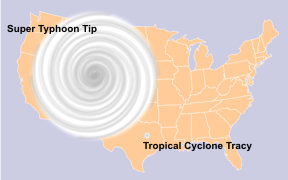
\includegraphics[width=15pc,angle=0]{typhoonsizes.jpg}
	\caption{Comparison of tropical cyclone sizes: Super Typhoon Tip and Tropical Cyclone Tracy. Source: \cite{noaa_structure}}\label{fig:cyclone_size}
\end{figure}

They are hugely variable in terms of size, illustrated in figure \ref{fig:cyclone_size}, where Tropical Cyclone Tracy (1974) covers just 0.03\% the area of Super Typhoon Tip (1979). Tropical cyclones tend to extend throughout the depth of the troposphere, approximately 16 km. The Saffir-Simpson Hurricane Scale \citep{simpson1974hurricane} is often used to categorise tropical storms by intensity based on maximum winds. Storms with winds of 38 mph (61 km/h, 33 knots) or less are called 'tropical depressions' and above this they are called 'tropical storms'. With increasing intensity there are categories 1 to 5 'hurricanes', with categories 3,4,5 referred to as 'major hurricanes'. In the West Pacific basin, if maximum sustained winds reach 64 knots (33 m/s, 74 mph) the term 'typhoon' is used, and a 'Super Typhoon' is if the maximum sustained winds are at least 130 knots (67 m/s, 150 mph).
The speed they move along the underlying surface, or 'translation speed' is around 10-15mph (10 knots), but can slower or as fast as 40 mph \citep{mo_tc}.  
%Size is not necessarily an indication of hurricane intensity. 


\subsection{Formation of tropical storms}

There are a number of environmental factors that need to be satisfied in order for a tropical storm to generate at a location. These are:
\begin{itemize}
	\item Presence of a convective system
	\item Non-negligible Coriolis force (at least 500 km, 300 miles) from the equator) \citep{noaaA15}
	\item Low wind shear (less than about 20 knots (10 m/s, 23 mph) \citep{noaaA15} 
	%	\item Enhanced vorticity
	\item Sufficient humidity in the mid-troposphere
	\item Warm ocean water of at least 26.5$^{\circ}$C throughout a sufficient depth (50m) (section 1.3.1)
	
\end{itemize}

Tropical cyclones cannot be generated spontaneously. To develop, they require a weakly organized system with sizeable spin and low level inflow. For tropical cyclogenesis to occur, there is a requirement for the Coriolis force to provide for near gradient wind balance to occur. Without the Coriolis force, the low pressure of the disturbance cannot be maintained. Large values of vertical wind shear disrupt the incipient tropical cyclone and can prevent genesis, therefore little wind shear is important. Relatively moist layers near the mid-troposphere (5 km, 3 miles). Dry mid levels are not conducive for allowing the continuing development of widespread thunderstorm activity. The development and maintenance of tropical cyclones require a warm ocean surface to act as a source of energy.

%Tory = enhanced cyclonic low-level vorticity .A pre-existing near-surface disturbance with sufficient vorticity and convergence. 
%Tropical waves spawn tcs... AEW, MT
%An atmosphere which cools fast enough with height such that it is potentially unstable to moist convection. 
%Tory - Tory - deep convection


\subsection{Tropical storm structure}

The main parts of a tropical cyclone are the dense cirrus overcast, rainbands, the eye, and the eyewall (figure \ref{fig:cyclone_structure}). There is boundary layer inflow in a cyclonic direction (anti-clockwise in the northern hemisphere) and anti-cyclonic (clockwise) upper tropospheric outflow.


\begin{figure}[h]
	\centering
	\noindent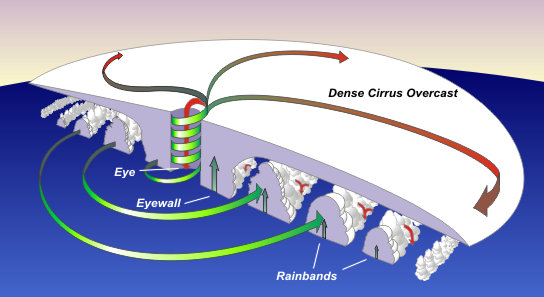
\includegraphics[width=20pc,angle=0]{hurr_cross.jpg}
	\caption{Tropical cyclone structure. Source: \cite{noaa_structure}}\label{fig:cyclone_structure}
\end{figure}

\subsubsection{Eye and eye wall}
The circular 'eye' or centre of a tropical cyclone is an area of slowly sinking air, characterised by light winds (usually do not exceed 15 mph (24 km/h)) \citep{noaa_structure} and little or no precipitation (figure \ref{fig:cyclone_structure}). Eye diameters are typically 40 km but can range from under 10 km to over 100 km \citep{bom_tc}. Although the winds are calm at the axis of rotation, strong winds may extend well into the eye. The eye is the region of lowest surface pressure and warmest temperatures aloft.

\begin{figure}[h]
	\centering
	\noindent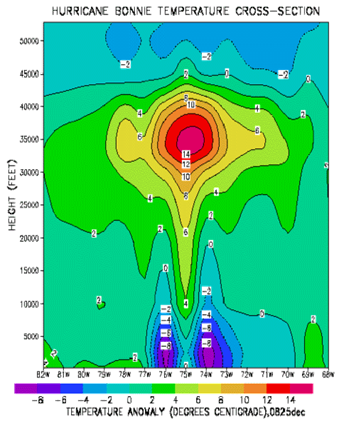
\includegraphics[width=14pc,angle=0]{warm_core2.png}
	\caption{Hurricane Bonnie temperature cross-section: the warm core. Source: \cite{eastin}}\label{fig:warm_core}
\end{figure}

Figure \ref{fig:warm_core} shows the maximum temperature anomalies present in the upper levels of the eye of Hurricane Bonnie. This is a result of subsidence and adiabatic heating in the eye, and eyewall latent heat release. The warm core is responsible for the extremely low surface pressures in the eye and large pressure gradients across the eyewall. The eye temperature may be 10$^{\circ}$C warmer or more at an altitude of 12 km (8 miles) than the surrounding environment, but only 0-2$^{\circ}$C warmer at the surface (Hawkins and Rubsam 1968) in the tropical cyclone (figure \ref{fig:warm_core}).

The eye is surrounded by a dense ring of cloud deep convection about 16 km high known as the eye wall which marks the belt of strongest winds and heaviest rainfall (\citep{bom_tc}). Changes in the structure of the eye and eyewall can cause affect the wind speed within the storm. The eye can grow or shrink in size, and double (concentric) eyewalls can form. In intense tropical cyclones, some of the outer rainbands may organize into an outer ring of thunderstorms that slowly moves inward. The inner eye wall (and storm intensity) weakens as it feels the effects of the subsidence resulting from this outer eyewall, inhibiting the inner eyewall of its needed moisture and momentum. Eventually the outer eyewall replaces the inner one completely and the storm can be the same intensity as it was previously or, in some cases, even stronger.% REF this section about weakening and intensifying. The pressure rises due to the destruction of the inner eyewall are usually more rapid than the pressure falls due to the intensification of the outer eyewall, and the cyclone itself weakens for a short period of time. 
%Some of the most intense tropical cyclones exhibit concentric eyewalls, two or more eyewall structures centered at the circulation center of the storm ( Willoughby et al. 1982,Willoughby 1990a ). Just as the inner eyewall forms, convection surrounding the eyewall can become organized into distinct rings. 

There remains some debate about the mechanism by which the eye forms \citep{noaa_a11}. It may be due to the downward directed pressure gradient associated with the weakening and radial spreading of the tangential wind field with height (Smith, 1980), or subsidence forced by latent heat release in the eye wall (Shapiro and Willoughby, 1982), or a combination of mechanisms.

%The exact mechanism by which the eye forms remains somewhat controversial. One idea suggests that the eye forms as a result of the . Another hypothesis suggests that the eye is formed when latent heat release in the eyewall occurs, forcing subsidence in the storm's center . It is possible that these hypotheses are not inconsistent with one another. In either case, as the air subsides, it is compressed and warms relative to air at the same level outside the eye and thereby becomes locally buoyant. This upward buoyancy approximately balances the downward directed pressure gradient so that the actual subsidence is produced by a small residual force.  \citep{noaa_a11}

%At around 74 mph (119 km/h) the strong rotation of air around the cyclone balances inflow to the center, causing air to ascend about 10-20 miles (16-32 km) from the center forming the eyewall. This strong rotation also creates a vacuum of air at the center, causing some of the air flowing out the top of the eyewall to turn inward and sink to replace the loss of air mass near the center.

\subsubsection{Rain bands}
Convection in tropical cyclones is organized into long, narrow rainbands which are oriented in the same direction as the horizontal wind (figure \ref{fig:cyclone_structure}). Along these bands, low-level convergence and upper-level divergence are at a maximum. Warm, moist air converges at the surface, ascends through these bands, diverges aloft, and descends on both sides of the bands. Subsidence is distributed over a wide area on the outside of the rainband but is concentrated in the small inside area \citep{noaa_a11}. As the air subsides, adiabatic warming takes place, and the air dries. Because subsidence is concentrated on the inside of the band, the adiabatic warming is stronger inward from the band causing a sharp contrast in pressure falls across the band since warm air is lighter than cold air. Because of the pressure falls on the inside, the tangential winds around the tropical cyclone increase due to increased pressure gradient and eventually the band moves towards the centre (Willoughby 1979, 1990a, 1995). 

% Eventually, the band moves toward the center and encircles it and the eye and eyewall form 

%What is the intensity of rain in a TC?


\subsection{Tropical cyclone energy and lifecycle}

Within a tropical cyclone, there are two distinct circulations referred to as 'primary' and 'secondary' (figure \ref{fig:cyclone_circ}). The primary circulation is what visibly characterises the phenomenon, with winds swirling cyclonically around the cyclone eye. The secondary circulation is the flow of air into the centre, ascending in the eye and then divergence at upper levels.

%\begin{figure}[h]
%	\centering
%	\noindent\includegraphics[width=20pc,angle=0]{H:/Documents/Admin/ESA/gradient_wind_balance.png}
%	\caption{Gradient wind balance in primary circulation of a tropical cyclone. Source: \cite{circ_pic}}\label{fig:cyclone_circ}
%\end{figure}
%% Do not cite circ_pic as this reference url has '%', which means all following references are missed

\subsubsection{Gradient wind balance}% and thermal wind balance}

The basic horizontal balance in a tropical cyclone above the boundary layer is between the sum of the Coriolis and centripetal forces, balanced by the horizontal pressure gradient force. This balance is referred to as gradient balance (figure \ref{fig:cyclone_circ}). %The centripetal force alters the original two-force geostrophic balance and creates a non-geostrophic gradient wind.
The classic theory for hurricane intensification relies on the inflow induced by the deep convection. However, as the vortex strengthens, the boundary layer becomes increasingly important \citep{under_hurr}.

%A symmetric tropical cyclone is in approximate thermal wind balance \citep{comet_tm}. The thermal wind is the difference between the geostrophic wind at two vertical levels and therefore represents the vertical wind shear of the geostrophic wind.

%what goes on in the boundary layer?
%http://www.goes-r.gov/users/comet/tropical/textbook_2nd_edition/navmenu.php_tab_9_page_2.4.1.htm

%The reason that different peak winds can result in different central pressures is caused by the fact that the radius, r, of the peak wind varies. A storm with 40 m/s peak winds with a 100 km RMW will have a much lower pressure drop than one with a 25 km RMW.

\begin{figure}[h]
	\centering
	\subfloat[1a]{\includegraphics[width=2.4in]{gradient_wind2006.png}}
	\subfloat[2a]{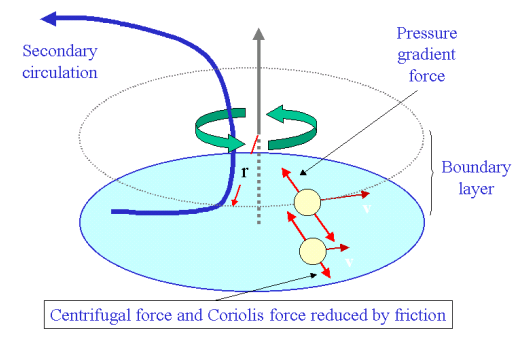
\includegraphics[width=2.4in]{gradient_wind2006B.png}}
	
	%	\noindent\includegraphics[width=20pc,angle=0]{H:/Documents/Admin/ESA/gradient_wind2006.png}
	\caption{a) gradient wind force balance in the primary circulation of a tropical cyclone b) disruption of gradient wind balance by friction in the boundary layer leaving a net inward pressure gradient that drives the secondary circulation with inflow in the boundary layer and outflow above it. Source: Smith, 2006}\label{fig:cyclone_circ}
\end{figure}

Surface friction in the boundary layer reduces the wind speed near the surface and therefore the centrifugal and Coriolis forces, but has little effect on the pressure field. There is therefore a new inward force in the boundary layer, driving inflow and the secondary circulation. The conservation of angular momentum means is objects will spin faster as they move toward the centre of circulation, so air increases its speed as it heads toward the centre of the tropical cyclone.


\subsubsection{Potential intensity}

To a good approximation, the secondary circulation in a tropical cyclone is a natural realisation of a Carnot heat engine, except that the engine does no work on its environment, the available work is locally dissipated and a fraction of the dissipated energy is recycled into the engine. A Carnot heat engine is the most efficient heat engine cycle allowed by physical laws. The Carnot perspective provides an upper bound on the maximum wind speed that a storm can attain.

\begin{figure}[h]
	\centering
	\noindent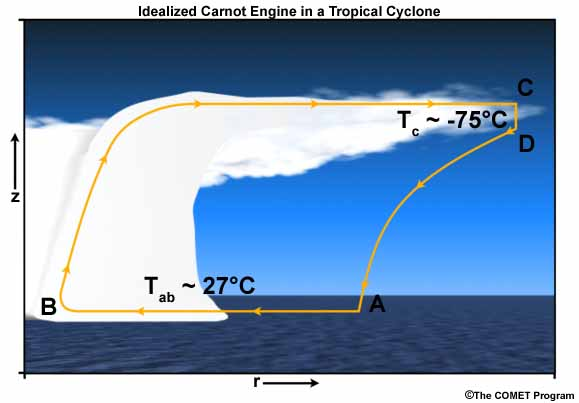
\includegraphics[width=20pc,angle=0]{carnot1.jpg}
	\caption{The Carnot cycle in a tropical cyclone. A-B: isothermal inflow of near-surface air; B-C: moist adiabatic ascent in the eye wall and outflow just below the tropopause; C-D: sinking of cooled air in the environment far from the tropical cyclone center. To close the system, D-A: the cooled air is assumed to return to the tropical cyclone environment adiabatically. Source:\cite{goescarnot}}\label{fig:cyclone_carnot}
\end{figure}

%CISK / WISHE
%\cite{emanuel1991theory} ref for carnot cycle
%vortical hot tower

%As this air ascends, 90\% of the stored energy is released by condensation, giving rise to the towering cumulus clouds and rain. The release of heat energy warms the air locally, causing a further decrease in pressure aloft. Consequently, air rises faster to fill this area of low pressure, and more warm, moist air is drawn off the sea, feeding further energy to the system. Thus, a self-sustaining heat engine is created.
%As little as 3\% of the heat energy may be converted into mechanical energy of the circulating winds. This relatively small amount of mechanical energy equates to a power supply of 1.5x1012 Watts - equivalent to about half the world-wide electrical generating capacity!
%http://www.metoffice.gov.uk/weather/tropicalcyclone/facts
%Emanuel theory 
%static vs dynamic theory

%In the northern hemisphere, positive vorticity at low levels and negative at upper levels. Vorticity decays with height. 

%It is the thunderstorm activity which allows the heat stored in the ocean waters to be liberated for the tropical cyclone development. (deep surface layer of conditional instability) - see Tory

%Intensification and decay
%Large vertical shear can weaken or destroy the tropical cyclone by interfering with the organization of deep convection around the cyclone center.
%(noaa website)
%maturity

%gray, frank montgomery, smith, tory book chapter- number of environmental conditions require to be satisfied for tc genesis.
%Emanuel
%ventilation
%Warm core is in thermal wind balance with the primary circulation.


\subsection{Steering of tropical storms} \label{steer}



%rotating winds of a tropical cyclone, combined with the north–south variation in the Coriolis parameter, induce relative vorticity asymmetries in the tropical cyclone (Fig. 8.60). These asymmetries are called the β–gyres.
%Tropical cyclones move in relation to the integrated, deep-layer (to \textasciitilde 17 km) environment flow in which they are embedded \citep{neumann1985role}.
% annulus degrees = see Carr 
%The motion of a tropical cyclone is highly correlated with latitude \citep{neumann1985role}. 
%5Chan 1985. (ref atm and ocean control sections). Low latitude easterlies and high lat westerlies, subtropical high.

A tropical cyclone is approximately 500-1000 km wide and 10-16 km high, set in much larger scale flow, so it can be treated as a solid object floating in the atmosphere \citep{chan2005physics}. Environmental steering is typically defined as the wind within an annulus centred on the tropical cyclone. e.g. 5-7 degrees (\citep{chan1982tropical}, \citep{chan1985identification} or 3 degrees (Franklin 1996). To define the steering flow, tropospheric layer means are better than single-level analyses \citep{velden1991basic}, with the deep layer mean (DLM)(1000-100 hPa) or mid-tropospheric level (500-700 hPa) often used. The vector quantity for the difference between the environmental steering and tropical cyclone motion is termed 'propagation' \citep{carr1990observational}. This difference arises from variations in the Coriolis parameter and environmental vorticity across the tropical cyclone. 

Depending on direction of movement of the storm, there is a different relationship with the surrounding flow \citep{chan1985identification}. Westward moving TCs move faster and to the left of the steering in the Northern Hemisphere, and eastward moving TCs move slower and to the right \citep{carr1990observational}.
%Importance of zonal direction of cyclone translation in determining the relationship between the environmental flow and cyclone movement. 

%Steered by surrounding flow and modified by Coriolis force (beta effect) and the horizontal vorticity gradient of the surrounding flow (chan physics review).
%NH Tcs move 10-20 degrees to the left and faster by 1ms than mid-tropospheric (700, 600, 500) at 6 degrees. 
%The beta effect - the cyclone and environment interact to modify the basic flow, and the vortex is then steered by this modified flow.

Studies have shown that depth of the steering layer is related to the strength of the cyclone \citep{velden1991basic}. For a more intense storm, there is greater vertical development of the cyclonic vortex, which is then advected by an environmental flow of greater depth. 

Tropical cyclone translation after landfall is affected by terrain, circulation environment, steering flow, TC intensity and structure among others \citep{xiao2013analysis}.
% effects of land, e.g. Philippines, Taiwan. track variation - interaction with topography (Wu and Kuo 1999), Taiwan


%Previous investigation into the sudden change in tropical cyclone track in four storms in the WNP suggested that such changes occurred near the centre of the MJO-scale cyclonic circulation or at the birfurcation of steering flows at 700 hPa \citep{wu2011observational}.

%Tropical cyclones forming between 5 and 30 degrees North latitude typically move toward the west. Sometimes the winds in the middle and upper levels of the atmosphere change and steer the cyclone toward the north and northwest. When tropical cyclones reach latitudes near 30 degrees North, they often move northeast

%Kim et al MJO effect
%Monsoon trough effect


\section{Impact of tropical storms}

Tropical cyclones are the most devastating natural hazards, affecting large populations in both the developed and developing world. Most of the damage occurs when tropical cyclones make landfall, and it is not only the destructive force of the strong winds, but also heavy precipitation and storm surge that cause widespread damage to communities.

Storm surges are responsible for much of the damage associated with landfalling tropical cyclones \citep{lin2012physically}. Storm surge is complicated, determined by the characteristics of the storms as well as shape and bathymetry of the coast, and the importance of the storm characteristics whilst over the open ocean and before landfall are also important. Rainfall distribution and intensity is complicated and depends on interactions on a variety of scales, with track, intensity, topography and environmental vertical shear all having an impact. Tropical storm wind fields change drastically when they make landfall, involving a complex interaction with the system and the underlying surface. The maximum damage of a tropical cyclone is not always at the point of landfall, but can be when it is further inland, for example when heavy rainstorms caused by interaction with mid-and lower-latitude systems once the storm is overland occur \citep{xiao2013analysis}. Although most damage occurs when tropical storms make landfall, they can also cause significant damage whilst at sea, mainly to the offshore industry. Loading on offshore structures is a complex function of not only characteristics of the wind field but also ocean characteristics including currents and waves \citep{done2014future}. Tropical-cyclone-wind resistant turbines have been deployed off the coast of China \citep{clark2014global}, to increase resilience to any future storms.

A recent notable tropical storm in the Western North Pacific is Super Typhoon Haiyan (2013). This is one of the most powerful typhoons ever to make landfall, with maximum sustained winds of 170 knots (88 m/s, 195 mph). Haiyan tracked over the Philippines archipelago, with storm surge primarily responsible for 6,300 dead, 1061 missing and almost 30,000 injured \citep{lagmay2015devastating}. %Average 472 fatalities a year (1983-2006) \citep{zhang2009tropical} 

Such landfalling typhoons also have a significant economic impact, for example Super Typhoon Herb (1996) caused 73.26 billion yuans  (£8.31 billion) in direct economic losses and became the costliest landfalling tropical cyclone in China at the time \citep{zhang2009tropical}. In China, there is an upward trend in the economic cost of landfalling tropical cyclones, and this is principally caused by economic development \citep{zhang2009tropical}.

%http://www.air-worldwide.com/Press-Releases/AIR-Estimates-Insured-Losses-from-Super-Typhoon-Haiyan-at-Between--USD-300-Million-and-USD-700-Million/

% From zhang2009tropical: In an average year, landfalling tropical cyclones cause 472 deaths and 28.7 billion yuans (2006 RMB) in direct economic losses, accounting for 0.38% of the annual total gross domestic product (GDP) of China. As the deadliest landfalling tropical cyclone, Super Typhoon Fred killed 1,126 people in 1994, making it the deadliest year (1,815 deaths). The costliest landfalling tropical cyclone was Super Typhoon Herb, which caused 73.3 billion yuans (2006 RMB) in direct economic losses in 1996, making it the costliest year (107.9 billion yuans). The direct economic losses and casualties of a landfalling tropical cyclone tend to increase with the northward shift in landfall track.



%%%%%%%%%%%%%%%%%%%%%%%%%%%%%%%%%%%%%%%%%%%%%%%%%%%%%%%%%%%%%%%%%%%%%%%%%%%%%%%%%%%%%%%%%%%%%%%%%%%%%%%%
\section{Tropical storm activity}

The Saffir-Simpson Hurricane Scale \citep{simpson1974hurricane} is often used to categorise tropical storms by intensity. Storms with maximum sustained winds of 38 mph (61 km/h, 33 knots) or less are called 'tropical depressions' and once over this threshold, are called 'tropical storms'. In the West Pacific basin, if maximum sustained winds reach 64 knots (33 m/s, 74 mph) the term 'typhoon' is used, and a 'Super Typhoon' is if the maximum sustained winds are at least 130 knots (67 m/s, 150 mph). %(http://www.srh.noaa.gov/jetstream/tropics/tc\_classification.html)
%(I need to remember if 1-min or 10-min. Which is US? Which is WMO?)

\subsection{Influence of the ocean} \label{ocean}

The ocean provides a source of energy to the tropical cyclone system by air-sea sensible and latent heat fluxes, determined by the sea surface temperature (SST). Many studies have shown that the SST must exceed 26$^{\circ}$C for tropical cyclones to form \citep[e.g.][]{palmen1948formation}. However, there is much research into this threshold \citep[e.g.][]{dare2011threshold, mctaggart2015revisiting}, highlighting basin-dependence and the importance of ocean temperature below the sea surface. The WNP has high SST throughout the year (\textgreater 28.5$^{\circ}$C) \citep{chan2007interannual}, relative to the suggested 26.5$^{\circ}$C threshold for genesis (section 1.2.1). Variability in activity is related to the SST pattern, with warm anomalies favouring intensification. The West Pacific is warm, past threshold limit, threshold more suitable for the North Atlantic, where more marginal.

The potential intensity of a tropical cyclone is directly related to the SST below the cyclone, all else being equal \citep{emanuel1991theory, holland1997maximum}, with higher SST promoting increased intensity. At high wind speeds, the surface wind stress generates strong turbulent mixing within the ocean. This causes entrainment of cooler water towards the surface from the thermocline and deepens the mixed layer.  The cooling of the SST is determined by the initial state of ocean, storm intensity, translation speed and storm size, and limits storm intensification, especially for slow moving storms, where SST cools more \citep{bender1993numerical, bender2000real}. During the lifetime of a storm, the wake produced can change considerably, for example Megi (2010) created a wake of 1.6$^{\circ}$C whilst in the Philippine Sea, but once in the South China Sea, cooling increased greatly to 7$^{\circ}$C \citep{d2014impact}. Due to this turbulent entrainment of cold water into the oceanic mixed layer induced by the TC, the state of ocean below the surface is also important to the cyclone system \citep{bender2000real, shay2000effects}.
%(see if any emanuel refs here - environmental control on...)
%Price 1981 - cooling 1 to 6C. \citep{price1981upper}
%Using satellites, observations of this cooling has been possible, 
%Cold wake of ~6C \citep{prasad2007upper}. 
%check Bender2000real.
%SST decrease induced by passage of a TC is approximately 1-6$^{\circ}$C  \citep{price1981upper}. 

The ocean heat content (OHC) in Joules (J) is a measure of the heat content within the ocean between two reference levels. 

\begin{equation}
OHC = c_{p} \int_{z1}^{z0} (T-T_{ref}) \rho dz
\end{equation} 	
%https://www.sharelatex.com/learn/Mathematical_expressions

%\begin{equation}
%$\displaystyle OHC = c_{p} \int_{z1}^{z0} (T-T_{ref}) \rho dz$
%\end{equation} 	

Tropical cyclone heat potential (TCHP) is vertically integrated heat content from the sea surface down to the 26$^0$C isotherm, which as at depth 'D26'.
% cannot find ref: as Gray (1968, 1978) suggested that depth of 60m is necessary for intensification.
%When this heat content is from the surface down to the 26$^0$C isotherm, it is termed tropical cyclone heat potential %(TCHP).
%Increased availability of sub-surface ocean observations, e.g. ARGO floats, since ...
%The ocean is the source of energy for a TC's intensification, typically down to 100-200m is important (Emanuel 1999) \citep{bender2000real}, \citep{shay2000effects}.
%Although WPAC SST is warm (generally above xyz), anomalously warm water can favour intensification. 

If the ocean warm layer (D26) is relatively shallow, (e.g. 60m) a positive SST anomaly is critical to intensification because the features can effectively deepen the warm layer and restrict the TC-induced cooling. If this layer is deep, e.g.\textgreater 105m, a warm feature is not required as the background is already sufficient to overcome the negative cooling feedback \citep{lin2008upper}.
%But isnt the warm SST anomaly needed in the first place?

In the WNP, intensification to category 5 needs SST around 29$^0$C and subsurface heat content required depends on the storm translation speed \citep{lin2009upper}. A shallow warm subsurface (D26 \textasciitilde 60m) is sufficient to intensify to a category 5 in a fast moving storm, but for slow moving storms, a much deeper warm layer is required \citep{lin2009upper}.

%Rapidly moving storms with deep oceanic mixed layer, SST feedback is of minor importance \citep{schade1999ocean}. All hurricanes attain their maximum intensity over warm ocean waters (does this mean the warmest or just above a threshold??) - from Prasad, referencing Goni and Trinanes, 2003

Typhoon Imbudo (2003) intensified from 56 knots (29 m/s, 65 mph) to 113 knots (58 m/s, 130 mph) in 12 hours when it passed over a region that increased TCHP by 100 kJ/cm$^2$. As the typhoon passed over these waters, the SST decreased by 3-4$^0$C alongside TCHP, but there was sufficient energy to negate the negative feedback of upwelling of cooler waters \citep{goni2003ocean}.
%But still there was cooling?


%On a much smaller scale, breaking waves and sea spray produced by TCs may change the wind stress \citep{moon2004effect}. Surface waves are a source of surface friction, moisture flux and ocean mixing and are a non-linear function of fetch and wind speed.

%Breivik et al. (2015) recently have demonstrated substantial improvement in climatological ocean biases with explicit treatment of surface waves. Waves generated by tropical cyclones are an important cause of infrastructure damage so an explicit and coupled treatment is desirable.

%%%%%%%%%%%%%%%%%%%%%%%%%%%%%%%%%%%%%%%%%%%%%%%%%%%%%%%%%%%%%%%%%%%%%%%


\subsection{Influence of the atmosphere}
%The atmosphere can maintain the TC or destroy it, principally through vertical wind shear.
A cyclone exists throughout the depth of the troposphere and so the atmospheric conditions have a large effect on the phenomenon. It has been established that vertical wind shear is detrimental to tropical cyclone genesis and intensification \citep[e.g.][]{chan1982tropical, McBride1995}, although mature, large tropical storms may resist relatively large wind shear \citep{zeng2007environmental}.

%One hypothesized pathway by which vertical shear affects tropical cyclones is mid-level ventilation, or the flux of low-entropy air into the centre of the tropical cyclone \citep{McBride1995}. Tropical upper tropospheric trough (TUTT) cells from the mid-latitudes can weaken tropical cyclones by introduction of vertical wind shear, but also bring a cyclonic PV anomaly, which may contribute to intensification \citep{zeng2007environmental}.
%EXPLAIN
%Strong vertical wind shear prohibits rapid intensification and most likely results in the weakening of TCs \citep{zeng2007environmental}.
%and a threshold of 12.5 ms$^-1$ above which TCs cannot form in the WPAC has been suggested \citep{zehr1992tropical}-seems to be a thesis - check this ref
%e and Zehr 1991, Zehr 1992 - thesis?)
%check zeng paper
% McBride and Tang for ventilation

The translation of TCs is largely determined by the large-scale atmospheric pattern, with mid-tropospheric levels (500 and 700 hPa) found to have the best correlation with TC direction and speed \citep{chan1982tropical} (\ref{steer}). If the passage of the storm is too slow, the cooling induced by the storm will inhibit intensification, and if it is moving too fast, the resulting asymmetric structure will also inhibit intensification \citep{zeng2007environmental}. Rapid intensification (RI) is An increase in the maximum sustained winds of a tropical cyclone of at least 30 kt in a 24-h period (\citep{nhc_gloss}). and for this to occur, a translation speed between 3-8 m/s is required. % (REF). % ref missing here

Although wind is the primary atmospheric control on TC activity, relative humidity and vorticity are also important.

% Fast translation speed and strong vertical shear and detrimental to TC intensification \citep{zeng2007environmental} and

%%%%%%%%%%%%%%%%%%%%%%%%%%%%%%%%%%%%%%%%%%%%%%%%%%%%%%%%%%%%%%%%%%%%%%%
\subsection{Tropical storm variability in the West Pacific}

Changes in atmospheric and oceanic conditions drive tropical cyclone variability. Tropical cyclone activity in most ocean basins including the WNP has a strong interannual signal \citep{landsea2000climate}, with variability observed in genesis location, track, intensity, landfall and lifetime.% (could use zhan2011contributions).

%Regions preferable for genesis. Or something like, genesis location is important and atmospheric conditions to maintain or dissipate storms are important. Distribution of SST important, also ocean at depth is important.

%(At the end mention interdecadal seasonal variability)

\subsubsection{El Ni\~{n}o}

It has been long established that the El Ni\~{n}o-Southern Oscillation (ENSO) (figure \ref{fig:nino}) is the principal driver of interannual variability in the Tropics. This phenomenon also has a marked effect on tropical storm activity in all basins. In a warm El Ni\~{n}o year, when the SST in the central and eastern equatorial Pacific is anomalously warm, there is a zonal displacement of annual mean tropical storm genesis location eastward \citep{lander1994exploratory, zhan2011contributions}. These storms tend to have a longer lifetime and can reach higher intensities before they recurve or meet land \citep{camargo2007cluster, chan1998seasonal}. In contrast, during La Ni\~{n}a years, the main region of genesis shifts westwards, with fewer intense storms.
%El Nino -weakening of Walker circulation. La Nina - strengthening.
%, Chan 2000, Wang and Chan 2002, for zonal displacement ENSO.


\begin{figure}[h]
	\centering
	\noindent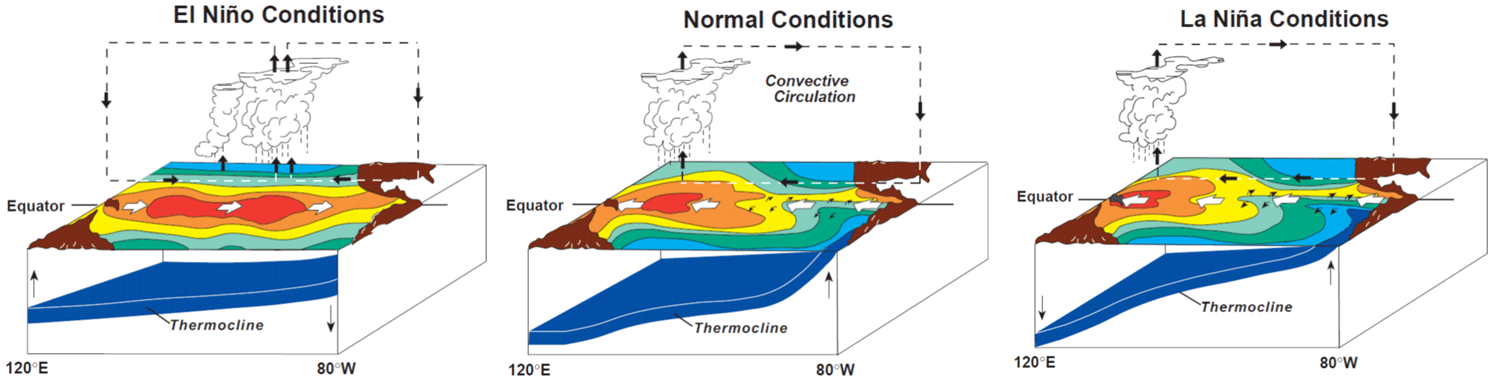
\includegraphics[width=40pc,angle=0]{Stressors_ENSO3.png}
	\caption{El Ni\~{n}o, normal and La Ni\~{n}a conditions in the atmosphere and ocean in the tropical Pacific. Source: \cite{noaa_enso}}\label{fig:nino}
\end{figure}


There is a significant difference in landfall location between El Ni\~{n}o and La Ni\~{n}a years. During El Ni\~{n}o, with more storms generated in the southeast quadrant of the WNP, they tend to recurve before landfall and affect Japan and Korea, with fewer across the Philippines and South China Sea \citep{liu2008interdecadal}. Whereas in La Ni\~{n}a years, the storms generate further westwards and are straight moving, with increased landfalls observed in China \citep{camargo2007cluster}.
%Does that mean that cyclones hitting China are weaker?

%ENSO affects the distribution of tropical storm numbers within the season \citep{lander1994exploratory}, as well as the landfall statistics, with \cite{yonekura2011statistical} finding significantly higher landfall rates in all coastal regions in La Ni\~{n}a.

%%%% MAKE FIGURE %%%%
% 	\begin{figure}[h]
% 		\noindent\includegraphics[width=20pc,angle=0]{Y:/Code_Data/Plots_NCAR/MAM/Maps/regions.png}
% 		\caption{Tropical storm tracks in 5 El Ni\~{n}o years and 5 La Ni\~{n}a years}\label{fregions}
% 	\end{figure}
% Look at Liu ZHou paper for years

Although El Ni\~{n}o has been shown to have a significant impact on tropical storm genesis location, the annual storm numbers have been shown to lack an ENSO signal \citep{lander1994exploratory}.

%ENSO - TC numbers: Chan 1985 too? Under debate - see zhan 2012.  However, El Ni\~{n}o has shown to have reduction in numbers - see Lander paper

%Wang and Chan (2002) observed an increase in the number of TCs in the WNP during strong El Ni\~{n}o events, though no significant linear relationship between TC number and indices of ENSO. A reduction in the number of TCs occurring in the summer following and El Ni\~{n}o has been found, related to Walker circulation (Chan 1985).

%The canonical eastern Pacific El Ni\~{n}o and the central Pacific El Ni\~{n}o have been shown to have different effect on TC activity in the Western Pacific (ref).

%In a study of intense typhoons, it was found that the interannual variations in the WNP were caused largely by changes in the planetary-scale atmospheric circulation and thermodynamic structure associated with El Ni\~{n}o \citep{chan2007interannual}.


\subsubsection{Other drivers of variability}

The Intertropical Convergence Zone, is the area encircling the earth near the equator where the northeast (N Hem) and southeast (S Hem) trade winds come together. Where the ITCZ is drawn into and merges with a monsoonal circulation, it is sometimes referred to as a monsoon trough. Most of the tropical cyclones that form in the WNP develop in the monsoon trough (MT) \citep{lander1994exploratory} and its location exhibits primary control on the distribution of TCs in the WNP \citep{wuinfluence}. 

\begin{figure}[h]
	\centering
	\noindent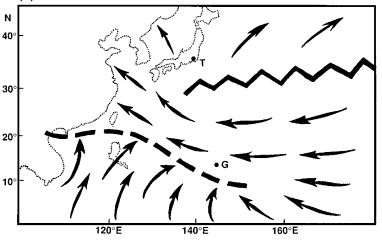
\includegraphics[width=20pc,angle=0]{MT_Lander.png}
	\caption{Long-term average of the low-level circulation during the summer in the Tropics of the western North Pacific. Bold zig-zag lines indicate ridge axes, and the bold dashed line indicates the axis of the monsoon trough. Arrows indicate wind direction. The locations of Guam (G) and Tokyo (T) are indicated. Source: \cite{lander1996specific}}\label{fig:MT}
\end{figure}

% when does the MT vary?
The monsoon trough is a climatological feature of low pressure and convergence (figure \ref{fig:MT}), with increased vorticity and it exhibits substantial migrations and changes of shape \citep{lander1996specific}. When the monsoon trough is defined as the contiguous region where long-term (1988-2010) mean July-November 850 hPa relative vorticity is positive, 73\% of all July-November tropical cyclones form within the monsoon trough \citep{molinari2013percentage}. This percentage displays interannual variation correlated with Ni\~{n}o 3.4 index, with more TCs forming in the MT in an El Ni\~{n}o phase \citep{molinari2013percentage}. The shift in genesis with ENSO phase has been related to the eastward extension of the monsoon trough and westerlies (associated with the increased cyclonic low-level vorticity) and the reduction in vertical wind shear near the date line \citep{lander1994exploratory, lander1996specific, wang2002strong}.
%See Camargo funny summary paper.
%Atmosphere - monsoon trough and subtropical ridge are important.See Harr and Elsbery 1991, 1995, Lander 1994, 1996, Liu and Chan 2002.

The Madden-Julian Oscillation (MJO) is a tropical mode of variability that has an intraseasonal time scale (30-90 days). It is characterised by an eastward progression of large regions of both enhanced and suppressed tropical rainfall, observed mainly over the Indian and Pacific Ocean. Over the western North Pacific (WNP), tropical cyclone activity appears to be strong when MJO related convection centre is in the WNP \citep{kim2008systematic}, however, no significant relationship with intensity has been found \citep{liebmann1994relationship}. As well as affecting the preferable region for genesis, TC tracks respond to the large-scale steering flows related to the MJO. When convection is in the equatorial Indian Ocean, tracks migrate eastward and when over the tropical WNP, they migrate westward \citep{kim2008systematic}.


%, Kim et al 1996.
%correct? See paper: Schreck et al (2012) 80-95\% WPAC TCs form in direct association with active MJO and/or active regions of various equatorial waves. 

%Studies have shown that the westerly phase of the Quasi Biennial Oscillation (QBO) corresponds to a larger number of TCs (refs) due to a decrease in the upper-tropospheric vertical shear over the tropics during the boreal summer. But does not hold during El Ni\~{n}o (See Chan 1995).

The subtropical high and mid-tropospheric flow pattern are important to TC movement \citep{chan1982tropical}. The strength and extend of the subtropical high influence where a TC will recurve (\ref{fig:STH}). %(ref steering section). How changeable is the sth?

\begin{figure}[h]
	\centering
	\noindent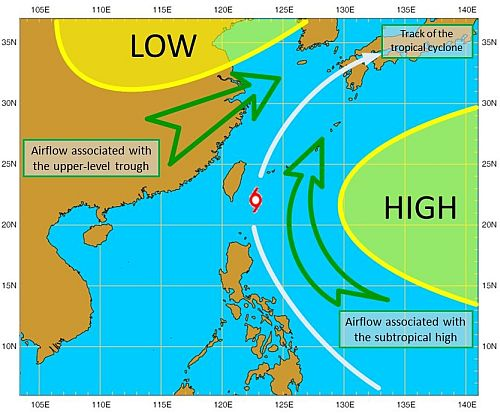
\includegraphics[width=16pc,angle=0]{typhoon16_1e.jpg}
	\caption{Subtropical High influence on TC movement. Source: }\label{fig:STH}
\end{figure}
%source http://www.weather.gov.hk/education/edu01met/01met_tropical_cyclones/ele_typhoon16_e.html

The Pacific Decadal Oscillation (PDO) exhibits variations in North Pacific SST over a decadal (20-30 years) timescale. It is similar to ENSO, with positive and negative SST anomalies, although it is on a much longer time scale and the most pronounced variations are at high latitudes, rather than in the Tropics  (figure \ref{fig:PDO}). The PDO Index is defined as the leading principal component of North Pacific monthly sea surface temperature variability (poleward of 20N for the 1900-93 period) (http://research.jisao.washington.edu/pdo/). The PDO has a significant impact on the subtropical high and mid-level steering during the peak TC season. It creates a north-south dipole of geopotential height over the WNP, affecting the subtropical high extension and intensity as well as the zonal winds \citep{liu2008interdecadal}.
%Check out Ho et al 2004 for PDO.
%NB wind stress changes with changing SST


\begin{figure}[h]
	\centering
	\noindent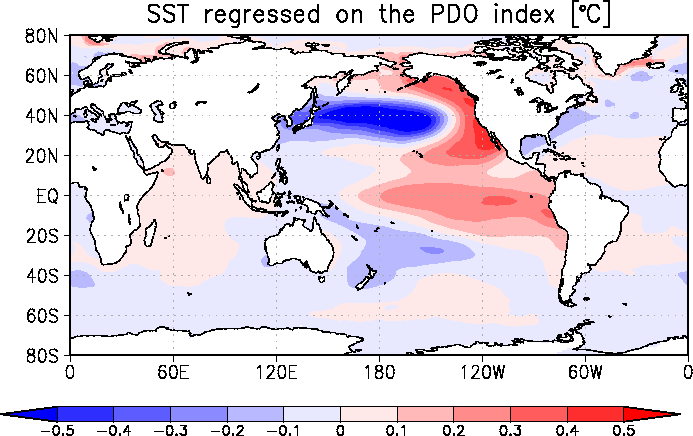
\includegraphics[width=20pc,angle=0]{pdo_pattern.png}
	\caption{Pacific Decadal Oscillation (PDO) positive phase. Figure from ADD SOURCE }\label{fig:PDO}
\end{figure}
%Add source to above: http://ds.data.jma.go.jp/tcc/tcc/products/elnino/decadal/pdo_doc.html


%WPSH is highly predictable and this can be used for tropical storm predictions \citep{wang2013subtropical}.

%Modes of variability - see Zhan 2012 review.
%Steering - Harr and Elsberry - straight, recurving, recurving north.
%IOD
%The intensity of a given storm depends on its surrounding environment.
%wang2013subtropical - Indian Ocean refs.

%Know about tropical waves - see Lu seasonal paper.

%IO importance - on MT?

Natural climate variability strongly modulates the seasonal statistics of tropical cyclones. 

%Affect of cyclone beforehand - upwelling is negative, but wave train is positive? (See camargo1)
%No - do not need to cover everything about TCs. Be specific and relevant.
%Something about historic activity can be divided into clusters, for example Camargo, Chan.

\subsubsection{Long-term variability}

Warming of the climate system is unequivocal \citep{stocker2013ipccb}, and as the internal energy available to weather systems such as tropical cyclones changes, activity of these phenomena is also expected to change. Warming of the ocean accounts for 93\% of the increase in the Earth's energy between 1971-2010, with 64\% of this in the upper ocean (0-700 m) \citep{rhein2013chapter}.

Modelling studies have consistently projected that greenhouse warming is likely to cause increases in the global average intensity of tropical cyclones and related rainfall rates \citep[e.g.][]{hill2011impact, knutson2010tropical, elsner2008increasing, bender2010modeled}, but some suggest that this is still within the range of natural variability. Many studies have shown that with an increase in SST in the coming decades, tropical cyclones will have increasing wind speeds \citep{bender2010modeled, murakami2012future, webster2005changes, emanuel2005increasing, knutson2010tropical, elsner2008increasing}, with \cite{emanuel2005increasing} suggesting that for every increase in SST of 1$^{\circ}$C, peak wind speed would increase by 5\%. The assumption is that the dominant effect of increasing carbon dioxide on tropical cyclones is through an increase in tropical mean sea surface temperature \citep{zhao2013robust}. However, modelling studies show that both spatial patterns of sea surface temperature warming and higher atmospheric carbon dioxide affect tropical cyclones independent of global sea surface temperature warming. % (ref)
% refs for within range of variability.
%The observed warming of the tropics of around 0.5$^0$C over the past 4 to 5 decades \citep{wang2010climate}. Consensus that the amount of energy will be the same, but higher lats will be increasingly exposed? \cite{huang2015change} suggested a suppressive effect of subsurface oceans on TC intensity in a warming environment due to sharpening of the subsurface vertical temperature profile, and therefore stronger ocean coupling (cooling).

Alongside SST warming, the effect of global sea level rise has consequences for damage caused by tropical cyclones. Global sea level has risen 10 to 20cm over last 100 years \citep{solomon2007climate} and it is very likely that the rate of global mean sea level rise during the 21st century will exceed the rate observed during 1971-2010 \citep{church2013sea}, so tropical cyclone-induced storm surge will become increasingly damaging phenomena. The water-holding capacity of air is a function of temperature, approximately doubling with each 10$^{\circ}$C increase in the range -20 to +45$^{\circ}$C \citep{fowler1995potential}. Therefore, in a warmer climate, precipitation from tropical cyclones will likely be more intense.

%That this rclationship is translated into pre¢ipitation potential is •vidcnccd by satdlitc obscrvations rcported by St•phcns (1990), which show a comparablc non-lincar rclationship b•tw••n s•a-surface tcmpcraturc and prccipitablc watet in a vcrtical air column ovcr the o¢cans. \citep{fowler1995potential}

%A number of factors that a warmer climate will affect on the activity and impact of tropical cyclones.

%Does it matter than here talking about modelling studies, before have talked about TCs in GCMs?

\section{Observations of tropical storms}
The historic record of tropical storm activity is longest for the North Atlantic, where records start in 1851 \citep{landsea2004atlantic}. Over the following decades, there has been a significant change in the methodology used to record such storms. In the early period, the main method for identifying tropical cyclones was by records of landfalling storms or by records of ships at sea \citep{vecchi2008estimates}. Further back in time, there were fewer ships and shipping lanes as well as fewer people living in the tropical and subtropical coastal regions \citep{landsea2007counting}, therefore it was possible that many storms were unrecorded. Aircraft reconnaissance in the West Pacific began near the end of the second World War and ended in 1987 \citep{knapp2013pressure}, and since then tropical storms have been monitored primarily by satellite \citep{lander1994exploratory}. The need for increased aircraft reconnaissance is acknowledged throughout the research and operational communities, with a recommendation from the World Meteorological Organisation (WMO) to 'realize the goal of regular and coordinated aircraft reconnaissance in the western North Pacific and other TC basins' \citep{wmoitwc8}. As part of government-led research, Japanese researchers are planning to have aircraft reconnaissance in the WNP from 2017 to at least 2020 \citep{nhkhurricanehunter}.

%, as many tropical cyclones(remove?)  were likely undetected over the tropical ocean in the pre-satellite era \citep{camargo2007cluster}

It is well established that although records begin many decades ago for some basins, they are only really trusted since the satellite era, ie. around the 1970s \citep{landsea2007counting} when global observations were possible. The observed time series of WNP tropical cyclone activity appears to be affected by artefacts of the changing observing system  \citep{lander1994exploratory, knapp2013pressure}, including the increasing use of satellite data and refining these methods, e.g. the Dvorak technique.
% and procedural changes . \citep{schreck2014impact} \citep{knapp2010international}

There are a number of agencies that produce Best Track records of tropical storm activity. The  International Best Track Archive Climate Stewardship (IBTrACS)\citep{knapp2010international} database consists of data from the World Meteorological Organization (WMO) Regional Specialized Meteorological Centres (RSMC) and Tropical Cyclone Warning Centres (TCWC) \citep{knapp2010international}. In the West Pacific region, data from the following agencies is available:

\begin{itemize}
	\item Fiji Meteorological Service (as RSMC Nadi)
	\item Japan Meteorological Agency (JMA) (as RSMC Tokyo)
	\item China Meteorological Administration’s Shanghai Typhoon Institute (CMA/STI)
	\item Hong Kong Observatory (HKO)
	\item U.S. Department of Defense Joint Typhoon Warning Center (JTWC)
\end{itemize}

For the WPAC region, JTWC storm data is most widely used \citep{knapp2010international}. All of the other agencies in this list provide data for a specific region in the West Pacific, rather than covering the entire basin. In some cases the same storms are tracked by multiple agencies, large differences in intensity can be found. There are also differences in lifetime as agencies employ different procedures for deciding when the first and last track point are determined.

%Modelling studies are vital, to learn more about TCs in the current climate and also to explore potential changes in the future.
% (tracks generallyu ok?), Also differences in lifetime - keep recording when goes ET or moves out of area of interest? Landfall in China goes further in CMA dataset (Matthias, pers comm). Different tracks, intensities, lifetime. eg. differences if calculating ACE. (see zhan2016cfs) Historical pressure record is more consistent between agencies than wind reports \citep{knapp2013pressure}.


\section{Representation of tropical storms in models}

\subsection{Global climate models}

Current CMIP5 (Coupled Model Intercomparison Project 5) models assessed in the IPCC Fifth Assessment Report (AR5) have a finest horizontal resolution in the atmosphere of around 70km, but the average is about 200km \citep{climodaus}, an increase from the previous four versions of the report.
It is well established that the current generation of global climate models (GCMs) are of insufficient resolution to simulate tropical cyclones in detail due to their low resolution in comparison to the size of the storm core \citep{lin2012physically} and the complex nature of tropical cyclone structure, although enhanced computing capabilities and parametrisations have resulted in better representation of tropical cyclones \citep{zhao2009simulations, bengtsson2007may, walsh2007objectively}.

Modern GCMs are capable of producing structures that can be recognized as similar to tropical cyclones at resolutions as coarse as 100 km (Knutson et al. 2010), but without the details of the core \citep{mcdonald2005tropical}. There is a need for very high resolution in order to simulate realistic storm intensities, \citep{bender2010modeled, emanuel2008hurricanes} for example it has been suggested that 2 km or less is needed to represent important physical processes in the tropical cyclone eyewall \citep{gentry2010sensitivity}, with \cite{chen2007cblast} suggesting that a resolution of 1 km is required to resolve hurricane eye wall convection and wind maxima.
%  (not realistic for GCM? Talking about RCM?)


Resolution is important for simulating storm intensity, but less critical for simulating the annual number of tropical cyclones and their geographical distribution. \cite{zhao2009simulations} found that a model with a resolution in 20-100km range was able to simulate climatology and interannual variability of tropical storm frequency without realistic distribution of storm intensity. Similar results were found by \cite{strachan2013investigating}, with realistic interannual variability of storm occurrence requiring resolutions of 100 km or higher, but skill was basin dependent. Different models produce substantially different annual global tropical cyclone frequencies and geographical distributions due to model resolution and physical parametrisations \citep{zhao2013robust}. It has been found that there are larger differences in tropical cyclone distribution between models than in the same model at different resolutions, suggesting a greater influence of model specifics than resolution \citep{shaevitz2014characteristics}.
%60km, 25 km, 12 km (NWP size).


%\subsection{Regional models}

%Regional models can be run at higher resolution than global models due to the reduced area over which calculations are being made. Typical resolution is ... and can be embedded in GCMs or GCMs downscaled.


%\newpage


\section{Seasonal prediction of tropical storm activity} % changed this from chapter to section

\subsection{Tropical storm forecasting techniques} % prediction?

%Remember focussing on climate, not NWP

The atmosphere is a chaotic system and so determinisitic predictability of weather phenomena, for example, tropical cyclones, is limited, and on a seasonal time scale, impossible. However, rather than forecasting exact cyclone tracks and dates of occurrence, predictions are made for basin-wide activity over a seasonal period.
Seasonal predictability of the climate system stems from the slowly evolving lower boundary, e.g. ocean forcing. The balance between the oceanic forcing and effects of random chaotic weather therefore determine the level of seasonal skill over a region \citep{rowell1998assessing}, and On a seasonal scale, atmospheric potential predictability is highest over the tropical oceans, where SST has an important effect, and this can be predicted using dynamical or statistical models \citep{rowell1998assessing}.
Seasonal tropical storm predictions are developed using dynamical, statistical, or statistical-dynamical models, with forecasts typically made 3 months ahead, e.g. March for the start of the season in June, with updated in May or June. 

%The time scales of changes in the ocean are much slower than in the atmosphere and can provide a source of predictability (e.g. ENSO). 
%The climate exhibits non-linear behaviour on a range of time scales, which may limit the seasonal climate predictability \citep{zhan2012seasonal}.
%, Palmer 2006.

%\begin{figure}[h]
%	\centering
%	\noindent\includegraphics[width=30pc,angle=0]{H:/Documents/Admin/ESA/seasonalforecasts.png}
%	\caption{Seasonal forecasts from different agencies. Most recent hurricane forecasts from each of the forecasting centers. Limits for the activity levels correspond to the ones defined by NOAA. Source: \citep{seasonalhurr}}\label{fig:seasonalforecasts}
%\end{figure}


%\begin{figure}[h]
%	\centering
%	\noindent\includegraphics[width=16pc,angle=0]{H:/Documents/Admin/ESA/na_ts_forecast_sm11.png}
%	\caption{Met Office seasonal forecast for North Atlantic. Also Hurricanes and ACE plots. None for the West Pacific yet as lacking skill. http://www.metoffice.gov.uk/weather/tropicalcyclone/seasonal/northatlantic2016}\label{fig:seasonalforecasts2}
%\end{figure}


%Predictable to some extent on seasonal time scale, but with large uncertainties. 
%predictability of large-scale environment


\subsection{Dynamical modelling}

In climate models accurate representation of the ocean is vital for climate simulation, especially over long periods, as the ocean represents a dynamic thermal reservoir that exchanges energy with the atmosphere. Fully-coupled atmosphere-ocean models, where heat and transport are fully represented and interactive, provide the best opportunity to capture relationships at a variety of scales.  These global models are vital as they can capture teleconnections, which are important for seasonal prediction. However, these are run at too coarse a resolution to capture the intensity. Model intensities are often not used directly, and instead are compared to the model climatology, which is then adjusted to cover the full spectrum of intensities. In order to extract the storms, a tracking algorithm needs to be applied to the model output. There are various different methods, for example tracking vorticity or minimum pressure, and then further thresholds are applied to select only tropical storms (e.g. warm core). %Tracking algorithms are not the same - not the same output storms, but with increasing resolution are better. Horn et al - thresholds. Basin-wide storm activity, released MAM? update June?


The skill of seasonal forecast models is often found to be higher using an ensemble than any single deterministic run \citep[e.g.][]{vitart2006seasonal}, and ECMWF use this ensemble approach. Dynamic models are important to explore the future climate, as long as they have sufficient skill at simulating the present climate and future forcings.

Seasonal forecasts for WNP tropical cyclone activity from dynamical models are produced by the European Centre of Medium-range Weather Forecasting (ECMWF). They have produced operational seasonal tropical cyclone forecasts for all basins since 2001 with their global coupled model. Predictions include tropical storm frequency, typhoon frequency, track density and accumulated cyclone energy (ACE) \citep{zhan2012seasonal}.

% Ensembles better than deterministic - see molinari cfs paper

%IRI uses\ a two step approach, whereby first SSTs are predicted using statistical or dynamical models, then atmospheric models are forced with these \citep{camargo12007seasonal}. IRI issues ACE forecast. IRI are probabilistic, normal , above normal, below normal \citep{camargo12007seasonal}. In both cases, TCs then tracked.
%ECMWF resolution
%IRI hybrid?????? , and the International Research Institute for Climate and Society (IRI). 
%Importance of ocean and ENSO prediction (refer to enso section). ENSO on SST field, but also on atmospheric pattern. Seasonal prediction of tc landfall represents a major challenge for dynamical models \citep{camargo12007seasonal}.\\
%\citep{rowell1998assessing} GCM skill in potential predictability
%\citep{vitart2006seasonal}
%\citep{mcdonald2005tropical}
%\citep{shaevitz2014characteristics}

%Limits of dynamical models for seasonal forecasting:
% \begin{itemize}
%	\item Resolution insufficient to capture storm structure and intensity (BUT there can be regional or hi res global dynamical models too?)
%	\item Global teleconnections need to be represented (and are they not?)
%	\item Model biases are present, which need to be corrected for
%	\item Limitations of the tracking methodologies (only apply to dynamical models?)

%\end{itemize}


%What are plans for operational - future - higher res, ensembles, physics problems to solve
%Landfall forecasts
%Modes of variability are important - teleconnections, also processes in the cryosphere, land, stratosphere, ocean, need fully coupled global  model.
%GloSea5, ECMWF and local models.
%bogussing? 

%basin wide and lead time 

\subsection{Statistical models}  
It has long been established that large-scale variability affects tropical cyclone activity globally. If a robust relationship between large-scale predictors and this activity can be found, it is possible to make predictions about future activity using statistical analysis.

The first region over which a statistical forecast for tropical cyclone activity was produced was the Australian region, in the late 1970s and 1980s \citep{nicholls1979possible, nicholls1985predictability}, with forecasts for the North Atlantic starting in 1984 \citep{gray1984atlantic}.

The first operational tropical cyclone forecasts for the West Pacific were issued by the National Climate Center (NCC) or CMA (China Meteorological Agency) in 1994 but these were only available in China \citep{zhan2012seasonal}. NCC currently issue seasonal forecasts of WNP tropical cyclone activity in March, with updates in June. The predictors are ENSO index, 500 hPa geopotential height over the Pacific and Australian region, convective activity over the WNP, vertical wind shear of zonal wind over the WNP and tropical eastern Pacific prior to the season \citep{zhan2012seasonal}.% EPAC Matters?

In 1997, The City University of Hong Kong, China (CUHK) started to issue seasonal forecasts to the public.  This scheme used SST anomalies as a proxy for ENSO signal, the large-scale circulation over Asia and the western Pacific, and trend or climatology and persistence \citep{chan1998seasonal}. New predictors related to ENSO including changes to the Southern Oscillation, Australian monsoon and subtropical high in the South Pacific have since been identified \citep{cl2001improvements}.
%persistence?
%Also did landfall in South China and Korea and Japan in 2009 and 2010 - still going?
%What is the CSL scheme? Does it stand for something? Not mentioned in the paper in 1998 - this is the one that details the model first used in 1997.
%(CHUK forecast 1997 or check this - is it 2000) The CSL scheme proposed by Chan et al 1998 
%.Relationship with the southern hemisphere related to the La Ni\~{n}a cold event.
Previous work by \cite{lu2013seasonal} examined the seasonal predictability of tropical cyclones affecting Taiwan using an empirical model. They found some skill in predicting accumulated cyclone energy (ACE) in the peak season (JJAS) using the SST in three regions and the sea level pressure (SLP) over an area in East Asia as predictors. 


%based on scientific understanding of the oceanic and atmospheric influence on tropical cyclones.
%Talk about verifying model using same dataset and similar region over Taiwan. Extending region to include more landfalling storms.

%Alongside CUHK and NCC, Tropical Storm Risk (TSR) also issue a statistical forecast for the WNP.
%statistical forecasts from CityU, National Climate Center China (NCC), Tropical Storm Risk (TSR) for the WNP. 

%Using a multivariate linear regression procedure, some skill is found using 3 regions of sea surface temperature and one region of sea level pressure predictors in forecasting the ACE over Taiwan. 
%Usually issued in March or April, with update in June or July.
%Seasonal statistical model - predictability from the spring to summer evolution of the monsoon subtropical high-ENSO system in association with the evolution of the Indo-Pacific SST anomalies \citep{lu2013seasonal}.

%Statistical modelling section - can also use statistical models of the large-scale environment to predict storm intensity distribution \citep{lee2015probabilistic}.
%Estimating or predicting landfall is important. Can create genesis models, track models etc. all from large-scale environment.

Limitations of such statistical forecasts include the dependence on historic observed data. this data is relatively limited (50 years) and has associated biases and errors. They assume stationarity of relationships and are unable to be used for climate change projections.
%Need to have cross correlations. Climate projections are difficult as rely on the signal at present (and in historic record).

%Limitations of statistical models for seasonal forecasting:
%\begin{itemize}
%	\item Dependent on historic observed data (limited and short record)
%	\item Climate projections difficult as future projections rely on present signal
%	\item Often assumes stationarity in relationships

%\end{itemize}

Alongside statistical and dynamical approaches, hybrid statistical-dynamical approaches have increased in popularity in recent years.

\subsection{Hybrid dynamical-statistical models}  
These models are a combination of the dynamical and statistical modelling approaches. A statistical model is developed based on either observations or output from a climate model seasonal prediction, and then this is applied to the seasonal prediction using predictors from a dynamical model. Skill of this model depends on robustness of the statistical relationship as well as the skill of the model to predict the predictor. \cite{zhan2016cfsv2} showed that a hybrid dynamical-statistical model showed better skill at longer lead times that the pure statistical model at predicting seasonal accumulated cyclone energy (ACE).
%BUt this PHd will focus on statistical?
% stationarity

%Quick summary sentence about timing of the forecast.
%ENSO predictability follows a cycle, where state for 4-6 months can be relatively accurately predicted between July and November \citep{camargo12007seasonal}. Once an episode has begun, predicting its continuation for the next 9-12 months is much easier than predicting its initial appearance \citep{camargo12007seasonal}.

%Relate this to TC season and timing of forecasts.

%\subsubsection{Seasonal forecast verification}  

%Previous studies have created statistical models of ACE or other tropical storm diagnostics such as frequency etc. (eg. Chan, Lu), and here we add to this by including the sub-surface ocean state in terms of ocean heat content and tropical cyclone heat potential.ADD LANDFALL
%provides more information over the depth of the ocean, important for intensity of the storms (ref intro).

Most seasonal projections are basin-wide. Here, we explore seasonal forecasts for a specific region of landfall and utilise current reanalysis datasets, including data on the deeper ocean. We also extend the lead time of predictability into the previous 15 months before the season.%....... Lu at al did the Taiwan region 6 months in advance. Others have focussed on basin-wide forecasts. EXTEND

%%%%%%%%%%%%%%%%%%%%%%%%%%%%%%%%%%%%%%%%%%%%%%%%%%%%%%%%%%%%%%%%%%%%%%%%%%%%%%


%How does my work compare to what has already been done.



\section{Characteristics of extra-tropical cyclones}

%
%\section{Characteristics of extra-tropical cyclones}
Extra-tropical cyclones are a dominant feature of the mid-latitudes, associated with strong winds, precipitation and temperature changes. An extra-tropical cyclone is a low pressure system that primarily gets its energy from a horizontal temperature gradient. They have frontal features, i.e. they are associated with cold fronts, warm fronts, and occluded fronts and in the northern hemisphere have winds counter clockwise. Like tropical cyclones, they transport heat and moisture from the Tropics towards the poles and they are embedded in mid-latitude westerlies, travelling in an eastward direction.

%what kind of intensities? named?

\section {Formation and structure of extra-tropical cyclones}
%Formation of jet streams? - no, not jet streams
%
%\begin{figure}[h]
%	\centering
%	\noindent\includegraphics[width=20pc,angle=0]{H:/Documents/Admin/ESA/jetstream3.jpg}
%	\caption{North hemisphere cross section showing jet streams and tropopause elevations. Source: \cite{noaa_jetstream}}\label{fig:jetstream}
%\end{figure}

The first conceptualised model of the typical life-cycle of mid-latitude cyclones is the Norwegian model (e.g. Bjerknes and Solberg). This was proposed in the 1910s and 1920s and describes the evolution of a cyclone from an incipient frontal wave with cold and warm fronts, through intensification, maturity and decay (figure \ref {fig:norwegian_maps}).

\begin{figure} % remove [h] and this appeared in the correct place
	\subfloat[Initial state]{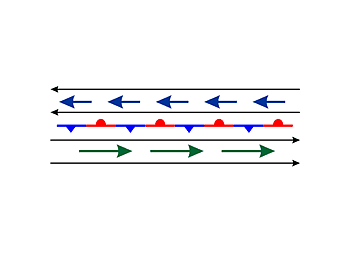
\includegraphics[width=2.0in]{cyclo1.png}}  % H:/Documents/Admin/ESA/Figures/
	\subfloat{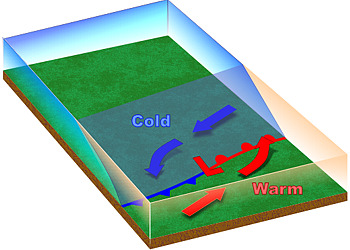
\includegraphics[width=2.0in]{wave23d.jpg}} 
	\subfloat[Beginning stage]{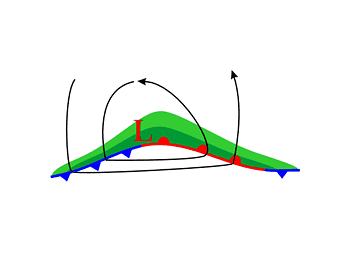
\includegraphics[width=2.0in]{cyclo2.png}} 
	\subfloat{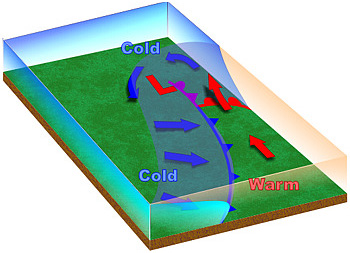
\includegraphics[width=2.0in]{wave43d.jpg}}  		
	\subfloat[Intensification]{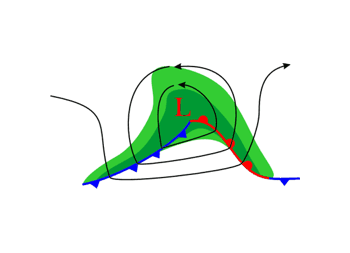
\includegraphics[width=2.0in]{cyclo3.png}} 
	\subfloat{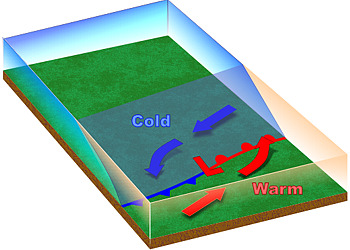
\includegraphics[width=2.0in]{wave23d.jpg}} 
	\subfloat[Mature stage]{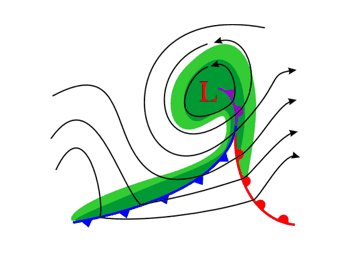
\includegraphics[width=2.0in]{cyclo4.png}} 
	\subfloat{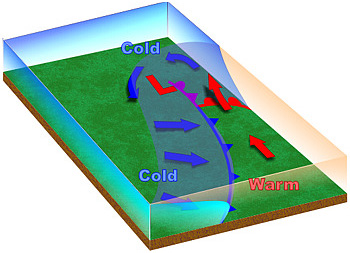
\includegraphics[width=2.0in]{wave43d.jpg}} 
	\subfloat[Dissipation]{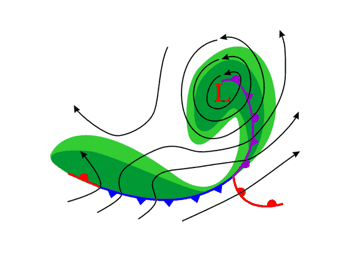
\includegraphics[width=2.0in]{cyclo5.png}} 
	\subfloat[]{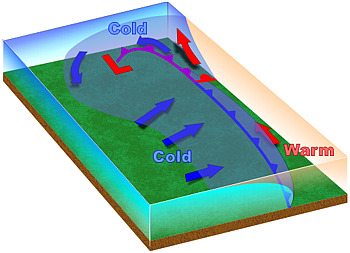
\includegraphics[width=2.0in]{wave53d.jpg}} 
	
	\caption{The Norwegian cyclone model in (1) map view (2) and 3-D view.  Source: \cite{norwegian}}\label{fig:norwegian_maps}
\end{figure}

One condition that favours cyclogenesis is a baroclinic zone, i.e. a region of large temperature change across a short horizontal distance near the surface, e.g. frontal zones. Above (near the tropopause) and parallel to this baroclinic zone is often a strong jet stream, driven by the thermal wind effect \ref{stull}. A wave develops on the front as an upper level low pressure system embedded in the jet stream moves over the front. As the air masses begin to rotate, defined cold and warm fronts develop. The wave intensifies and the low pressure centre deepens. The warm sector narrows as the cold front rotates around the cyclone faster than the warm front, and an occluded front develops where the cold front overtakes the warm front. As the cold front continues advancing on the warm front, the occlusion increases and eventually cuts off the supply of warm moist air, causing the low pressure system to gradually dissipate \citep{norwegian}. Precipitation occurs as air is forced to rise ahead of the warm front and the cold front. The more dense cold air undercuts the warm air and the less dense warm air rises above the cold air.

%http://weatherfaqs.org.uk/node/98
%As with the Norwegian cyclone model, the Shapiro-Keys model has an incipient cyclone develops cold and warm fronts, but in this case, the cold front moves roughly perpendicular to the warm front such that the fronts never meet, the so-called 'T-bone'. Also, a weakness appears along the poleward portion of the cold front near the low center, the so-called 'frontal fracture' and a back-bent front forms behind the low center. (In the final stage), colder air encircles warmer air near the low center, forming a warm seclusion. 

An alternative model is the Shapiro-Keyser model. The main difference from the Norwegian model is that the cold front moves roughly perpendicular to the warm front and they never meet. The occluded front is due to a weakness in the cold front near the low centre.
%The occluded front is an extension of the warm front rather than a result of the cold front catching up with the warm front. Both are valid and suited to different scenarios.. e.g....

%Conditions favourable to cyclogenesis are a baroclinic atmosphere (a region of large temperature change across a short horizontal distance near the surface), there is often an associated a strong jet stream running parallel at upper levels.
%what about mositure?
%cyclogenesis involves sea-level pressure decrease as the low pressure centre deepens, upward-motion increase, and vorticity increase.

Energy from baroclinicity in the atmosphere. This is in contrast to tropical cyclones, where there is little temperature contrast across them and they get their energy from the underlying ocean. Much like tropical cyclones, extra-tropical cyclones are moved by the jet stream and by other large-scale components of the global circulation \citep{stull}.

%Baroclinic instability is due to a horizontal temperature gradients in a rotating environment. 

%What season? winter storms or summer storms? extratropical transition?

%extratropical ocean-atmosphere interaction dominated by atmosphere forcing the ocean, but with variability with oceanic processes more important to SST in the vicinity of WBCs (smirnow).

%baroclinic wave, steering level. Steered by large scale, much like TCs?

Figure \ref{fig:ET_structure} shows a mature extra-tropical cyclone in more detail. An extra-tropical cyclone is typically larger than an average tropical storm, (approximately 1000 km)
As an extra-tropical cyclone moves eastwards, ahead of the warm front, there stratiform cloud as warm air is forced to rise and cool. Behind the warm front is the warm sector, of relatively warm air and generally clear skies. At the cold front, dense cool air undercuts the warm, moist air and forces it steeply upwards, with a band of cumuliform clouds, heavy rain and thunderstorms. Following the passage of the cold front, there is cooler air, bright skies and showers, and a marked veer in wind direction. The near surface winds converge towards the low pressure centre. Structurally, extra-tropical cyclones are 'cold-core', unlike tropical cyclones, which are 'warm core'.
%Cold sector surface flow is from the northwest
%Warm sector surface flow is from the southwest, bringing warm low-latidude air poleward and upward 'warm conveyor belt', associated with weak turbulent heat fluxes at the surface (warm path pahper?). Warm conveyor belt, cold conveyor belt, dry intrusion.

\begin{figure}[h]
	\centering
	\noindent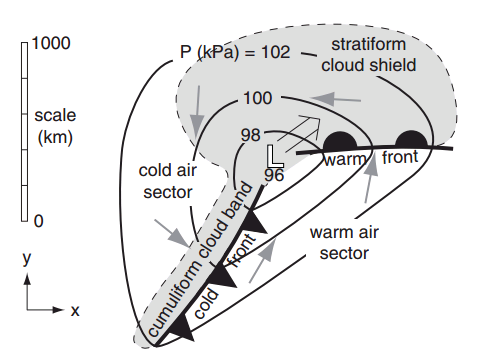
\includegraphics[width=20pc,angle=0]{ET_structure.png}
	\caption{Components of a typical extra-tropical cyclone in the N. Hemisphere. Light grey shows clouds, dark grey arrows are near-surface winds, thin black lines are isobars (kPa), thick black lines are fronts, and the double-shaft arrow shows movement of the low centre 'L'. Source: \cite{stull} }\label{fig:ET_structure}
\end{figure}


%\section {Impact of extra-tropical storms}

\subsection {Extra-tropical storm activity} %ocean, atmos, variability
%
Much like with tropical cyclones, the variability of extra-tropical storm activity is due to both atmospheric and ocean conditions. These storm systems extend through the atmosphere, however, underlying conditions in the MBL are important too. The marine boundary layer (MBL) is the part of the atmosphere that lies over the ocean surface and is directly influenced by it.  Variations in the ocean surface therefore affect the cyclone, affecting ocean-atmosphere exchanges of heat, moisture and momentum.

%Due to variations in the atmosphere and ocean - baroclinic atmosphere required for cyclogenesis (ref section). 

Extra-tropical storms are driven by strong temperature gradients (section 3.1) and in the North Atlantic, often develop in baroclinic zone over Gulf Stream. In the MABL, the Gulf Stream directly influences air temperature and pressure fields but also has effects throughout the entire troposphere, with upper-tropospheric divergence exhibiting a structure similar to the surface convergence and precipitation patterns, all meandering with the Gulf Stream (\citep{minobe2008influence}).
%Major storm tracks are organised along or just downstream of the main oceanic frontal zones (Nakamura et al 2004).
%Sheldon(The atmosphere above the Northern Hemisphere’s western boundary currents (the Gulf Stream and Kuroshio) are maximums in the winter atmospheric variability on a synoptic timescale of 2-6 days (Lau and Wallace, 1979; Blackmon, 1976; Hoskins and Valdes, 1990). These regions of synoptic variability are called the storm tracks and the variability is measuring the growth of extra-tropical cyclones that occur there (Dacre and Gray, 2009).)

In the marine atmospheric boundary layer (MABL), the Gulf Stream directly influences air temperature and pressure fields locally and also throughout entire troposphere, with upper-tropospheric divergence exhibiting a structure similar to the surface convergence and precipitation patterns, all meandering with the Gulf Stream (\cite{minobe2008influence}). Extra-tropical storms are driven by strong temperature gradients and in the North Atlantic, often develop in the baroclinic zone over Gulf Stream. Here, strong oceanic fronts that help to maintain the strong baroclinicity that is required to maintain them \citep{nakamura2004observed, nakamura2008importance, hoskins1990existence}

%\cite{nakamura2004observed}
%As the surface air temperature over the open ocean is linked to SST underneath, maritime surface baroclinic zones tend to be anchored along oceanic fontal zones [NS04]. Though acting as thermal damping for the evolution of individual  eddies, heat exchange with the underlying ocean, on longer time scales, can act to restore atmospheric near-surface baroclinicity against the relaxing effect by atmospheric eddy heat transport, as evident in sharp meridional contrasts in upward turbulent heat fluxes observed climatologically across midlatitude frontal zones [Oberhuber, 1988]. Some observations are shown in section 2 to suggest that SST anomalies in a midlatitude frontal zone can likely play a more active role in the air–sea interaction than act to damp  tmospheric anomalies thermally Hoskins and Valdes (1990) mean diabatic heatin as a result of the warm ocean current restores the meridional atmostpheric temperature gradient and therfore baroclinciiy, that is vital to the storm tracks existence.

%nakamura et al 2008 \cite{nakamura2008importance}
%and booth et al 2010 - air-sea heat exchanges at oceanic fronts restore the baroclinicity of the atmosphere at low levels.
%shear instability not parametrised in current generation of GCMs.

%GCMs generally simulate the storm tracks well (d'Andrea et al 1998)as they are large-scale phenomenon of the atmospheric circulation. Also climate models can capture the structure of ETCs (cite{\catto2010can}).
%Atmosphere-ocean interactions are their strongest over WBCs, e.g Gulf Stream. Strong fluxes of heat and moisture anchor the storm tracks to the WBCs (Nakamura et al 2004). allows for recurrent develpoment of storm tracks - creates baroclinicity?

%Deep ascent over the Gulf Stream is a result of extreme events, i.e. extra-tropical storms \citep{minobe2008influence}(check this)
%The storms occur in these locations as the strong oceanic fronts help maintain the surface baroclinicity required to produce them (Nakamura and Shimpo, 2004 Nakamura et al., 2008; Sampe et al., 2010).  (sheldon thesis).
%SHELDON THESIS:
%The Gulf Stream is the western boundary current for which the most links to deep convection have been found. %The deep ascent over the Gulf Stream found by Minobe et al. (2008) is a result of extreme events that skew the mean to ascent, and their results do not represent an average day in that region. The ascent above the Gulf Stream being a product of extreme events is consistent with the region also being the centre of action for winter synoptic systems in the Northern Hemisphere (Hoskins and Valdes, 1990).


\subsubsection {The Gulf Stream}

Global atmospheric circulation is characterised by easterly trade winds in the Tropics and the westerlies in the mid-latitudes.  The atmosphere exerts a force on the ocean below, which is also affected by the rotation of the earth, a factor which increases with proximity to the poles. Surface currents located on the western side of ocean basins are must faster than on the east and are among the fastest surface currents in the ocean (\citep{nasa_ocean}).  These currents also extend much deeper than most other surface currents, and are deflected by the continental margins, which prevent these currents from flowing onto the shallow continental shelves \citep{nasa_wbc}.
%Waters in western boundary currents (WBCs) typically move 40 to 120 km (25 and 75 mi) per day (\citep{nasa_wbc}). 
The Coriolis effect increases with latitude, and so is stronger in the latitudes of the westerlies than in the latitudes of the equatorial trade winds. Surface waters build up on the western side of ocean basins, resulting in the ocean-surface slope to be steeper on the western side (versus eastern side), which leads to a faster geostrophic flow on that side \citep{nasa_wbc}.

The Gulf Stream can be seen in Sea Surface Temperature data (SST), transporting a warm tongue of water poleward and eastward (figure \ref{fig:GS_map}). On the northern edge, there is a strong SST gradient while to the south, eddies tend to erode this gradient.

\begin{figure}[h]
	\centering
	\noindent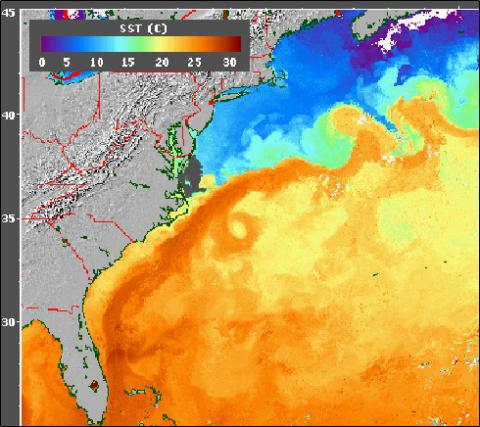
\includegraphics[width=14pc,angle=0]{GulfStream.jpg}\\ % H:/Documents/Admin/ESA/Figures/
	\caption{The Gulf Stream, revealed through SST data, made from the AVHRR (Advanced Very High Resolution Radiometer) sensor carried on a NOAA satellite. In this image, purple and blue represent the coldest temperatures (between 0-15 $^0$C) and orange and red represents the warmest temperatures (between 22-32 $^0$C). Source: \cite{gsnasa}}\label{fig:GS_map}
\end{figure}


%Deep ascent over the Gulf Stream is a result of extreme events, i.e. extra-tropical storms \citep{minobe2008influence}(check this)

It has been found that these extra-tropical storms occur in locations such as the Gulf Stream, where there are strong oceanic fronts that help to maintain the strong baroclinicity that is required to maintain them (Nakamura and Shimpo, 2004 Nakamura et al., 2008).
%The storms occur in these locations as the strong oceanic fronts help maintain the surface baroclinicity required to produce them (Nakamura and Shimpo, 2004 Nakamura et al., 2008; Sampe et al., 2010).  (sheldon thesis).

%heat from the tropics poleward - affects cyclogenesis (how is this related to temp?)


\subsection{The warm path}

Previous studies \cite{vanniere2017cold} \cite{sheldon2017warm} have suggested a new mechanism by which the SST distribution of the Gulf Stream impacts cyclones over the North Atlantic Ocean. The mechanism consists in an intensification, and possibly a destabilization, of the frontal circulation embedded in the cyclones. 

The 'warm path' is the mechanism of oceanic forcing  associated with impact of the Gulf Stream warm tongue on the warm sector of cyclones. Here there are weak air-sea heat fluxes, which is in sharp contrast to what occurs in their cold sector.

In \cite{sheldon2017warm} , this warm path mechanism has been examined using one case study on January 14th 2004, with a MetUM simulation (12km) integrated for 72 hours. A 'SMTH' experiment used a smoothed Gulf Stream warm tongue SST, a 'COOL' reduced the SST everywhere by 3K and the control used an unperturbed SST. Results showed that the Gulf Stream has a significant impact on the upward motion present in the cyclone, with back trajectories providing a useful tool. 

\begin{figure}
	
	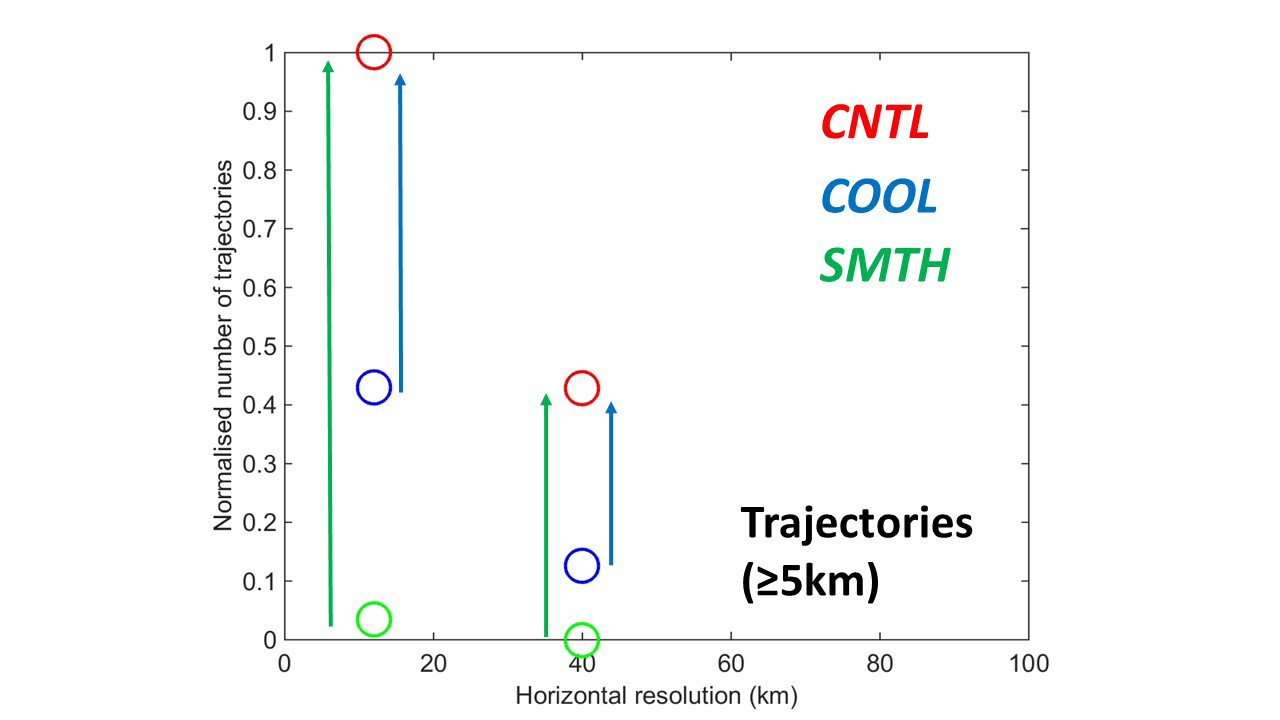
\includegraphics[width=22pc,angle=0]{warmpath_result.png} % H:/Documents/Admin/ESA/Figures/
	\caption{Number of back trajectories (circles) with heights z 5km at t=24h and reaching low levels over the ocean at t=0h: red for CNTL, blue for COOL and green for SMTH. The arrows indicate a measure of oceanic forcing when comparing CNTL,SMTH or CNTL,COOL. Normalized such that the number for CNTL at 12km resolution is unity. Source: Sheldon et al. 2016}\label{fig:wp_result}
	\centering
\end{figure}

Figure \ref{fig:wp_result} shows that at both model resolutions (12 km and 40 km), the control simulation has more than double the number of trajectories that the perturbed simulations, with the smooth simulation having a the fewest. Oceanic forcing is measured by the number of trajectories as this is related to upward mass transport, which scales with the diabatic heating (due to condensation of water vapour carried in the flow) in the ascending branch (Sheldon et al., 2016).

Thermodynamic and dynamic mechanisms have been proposed. For the thermodynamical mechanism, in the control experiment trajectories are parallel to the Gulf Stream, with no significant loss of heat and possible gain of moisture, maintaining high $\theta$e values. In the smooth simulation, air parcels cross SST contours, reducing $\theta$e and the likelihood of ascent. The dynamical considerations are that, due to stronger SST gradients in the control experiment, a thermally driven cell enhances the frontal circulation, increasing the feed into the warm conveyor belt. Also, it is possible that the stronger SST gradients destablise the frontal circulation by enhancing the vertical wind shear (Sheldon et al., 2016).

%Partitioning between bottom or top heavy feeding of the ascent from low levels is primarily set by SST gradient. Ability for air parcels to ascent in the WCB sensitive to the absolute SST.

%Dynamical diagnostic in ERA-Interim, suggests Gulf Stream warm tongue should have most frequency vigorous ascent from low levels in the NW Atlantic in winter.
%Climatological distribution of WCBs in the NH winter peaks over the Gulf Stream warm tongue.

This study \cite{sheldon2017warm}  focussed on one case study, and it will be valuable to explore this mechanism in more cases. Also just one model realisation, so examine other models (ref chapter) and other cases (ref chapter).


%Climate models (HiGEM (0.83x1.25) and ERA-40) can capture the structural features of extra-tropical cyclones \citep{catto2010can} analysing warm conveyor belt, cold conveyor belt and dry intrusion.

Explain in depth PV and equivalent potential temperature\\


\subsection{Atmospheric instability and convection}

\subsubsection {Gravitational instability and upright convection}

In a hydrostatically balanced atmosphere, the mean-state potential temperature ($\theta$) decreases with height. If the potential temperature cools with height, there will be overturning as the cool air sinks. This is gravitational instability (\ref{eqgravinst}), which releases upright convection and is purely vertical.

\begin{equation} \label{eqgravinst}
\frac{d\theta}{dz} < 0
\end{equation}


\subsubsection {Inertial instability and horizontal movement}
Inertial instability operates in the horizontal plane and is detected by absolute momentum (M). Absolute momentum, as defined by \cite{eliassen1962vertical} is the rotation of the Earth plus the rotation due to variations in the wind field:

\begin{equation} \label{eqM}
M = V + fx
\end{equation}


%\begin{equation} \label{eqN}
%N = U - fy
%\end{equation}

where V is the frontal velocity and x is the distance along the transverse plane to the front. When the absolute momentum decreases in the x-direction then the atmosphere is unstable:

\begin{equation} \label{eq_iner_inst}
\frac{dM}{dx} < 0
\end{equation}


\subsubsection {Shear (symmetric) instability and slantwise convection}

Shear (or symmetric) instability is a combination of gravitational and inertial instability. A parcel may be inertially stable to horizontal displacements and gravitationally stable to vertical displacements, but may be unstable to slantwise displacements by shear instability. 

A barotropic atmosphere is one where the density depends solely on pressure, whereas in a baroclinic atmosphere the density depends on both the temperature and the pressure. In a barotropic flow, potential temperature surfaces (isentropes) are horizontal and absolute momentum surfaces (M) are vertical. In a baroclinic environment, the isentropes tilt upwards on the cold side and downwards on the warm side. The absolute momentum surfaces slope in response to the vertical shear from thermal wind balance, tilting up on the cold side and down on the warm side.
%
%\begin{figure}[h]	
%	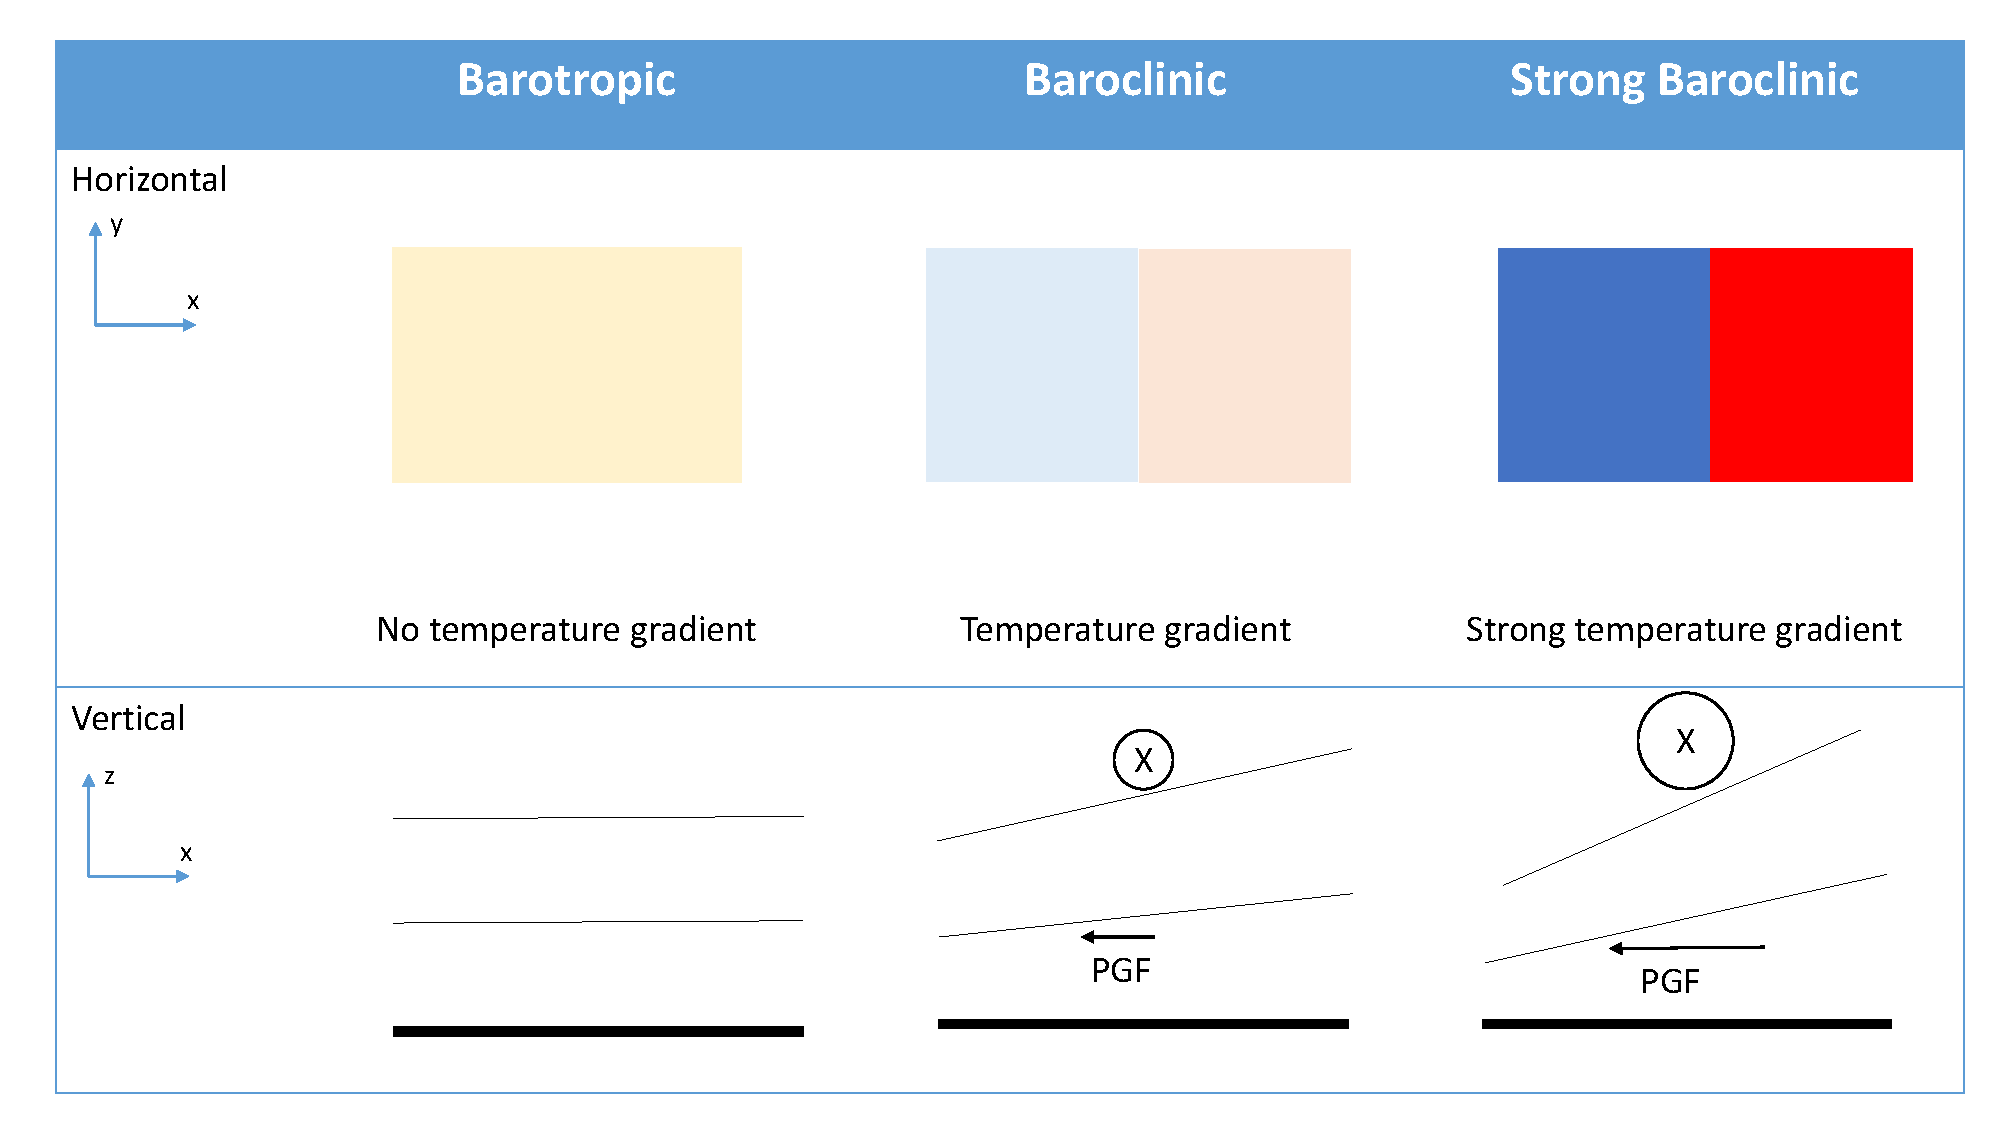
\includegraphics[width=34pc,angle=0]{H:/Documents/Thesis/phd-thesis-template-2.2.2_AC/phd-thesis-template-2.2.2/Figs/barotropic2_new.pdf}
%	\caption{Barotropic and baroclinic environments in the horizontal and vertical, and resultant pressure gradient force (PGF) and thermal wind (cross in circle). Thin black lines are isentropes.}\label{fig:barotropic}
%	\centering
%\end{figure} 

The  M-$\theta$e relationship states that if the $\theta$e surfaces are steeper than the M surfaces, there is symmetric instability. Any slantwise displacement occurring between the slopes of these surfaces will release the symmetric instability and the parcel will be accelerate in the direction away from the original position. Figure \ref{fig:symm_inst} illustrates the M-$\theta$e relationship, with a symmetrically unstable atmosphere on the left and a symmetrically stable atmosphere on the right. Only moist slantwise instability occurs in the Earth's atmosphere \cite{bennetts1979conditional} and so $\theta$e is used. This instability has a 2D assumption that there is no variation in the along front direction. 


\begin{figure}
	\centering	
	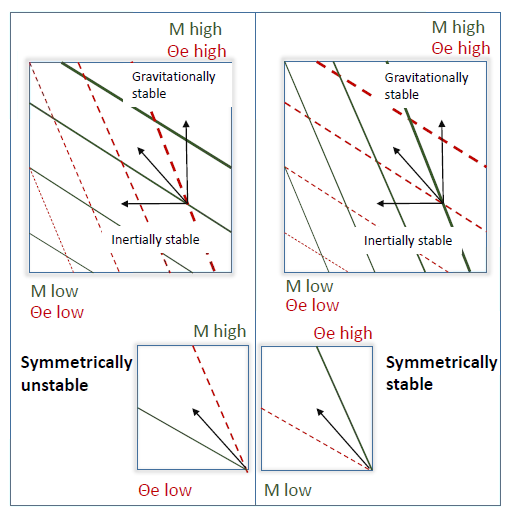
\includegraphics[width=26pc,angle=0]{mocrette_diagram2_screen.png}
	\caption{Shear (symmetric instability). Isentropes are shown in red dashed lines and lines of constant absolute momentum (M) in solid green. Thickness of the lines increases towards  higher values. Both environments are baroclinic and $\theta$e and M are low in the bottom left and high in the top right. The black arrows show direction of movement of air parcels. In both panels a and b, if a parcel is moved to the left, it is inertially stable as it is moving towards an area of reduced absolute momentum. In both panels a and b, if a parcel is moved vertically, they are gravitationally stable as potential temperature is increasing in this direction and so the parcel will return to it's original position. However, in panel a, if an air parcel is moved along arrow x, it is moving towards lower potential temperature and high M, so is symmetrically unstable. In panel b, it will move towards higher $\theta$e and low M, and is symmetrically stable. Modified from \cite{morcrette2004radar}}\label{fig:symm_inst}
\end{figure}


%\begin{figure}
%	\centering	
%	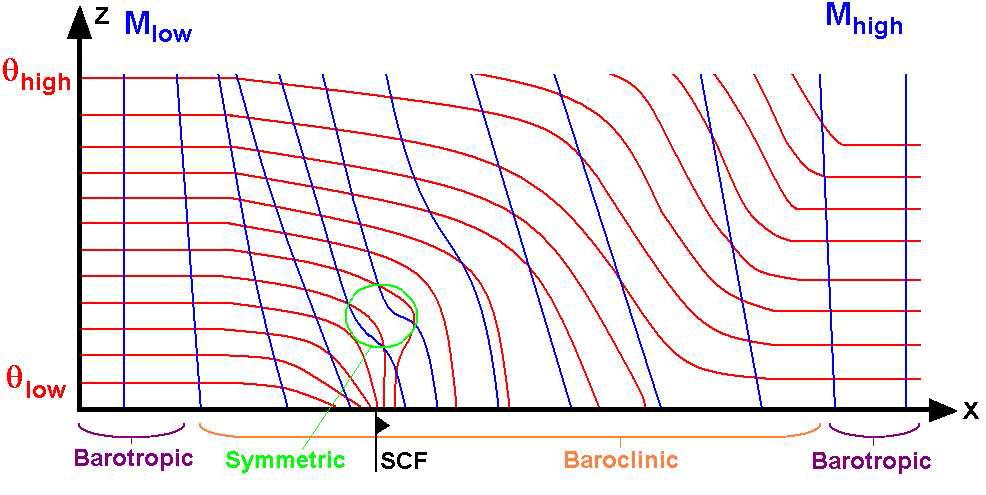
\includegraphics[width=26pc,angle=0]{H:/Documents/Thesis/phd-thesis-template-2.2.2_AC/phd-thesis-template-2.2.2/Figs/morcrette_cx.png}
%	\caption{1.6 The distribution of saturated equivalent potential temperature (red lines) and
%		geostrophic absolute momentum Mg (blue lines) in the broad region around a cold front. Far
%		from the front, the atmosphere is barotropic, within the cold frontal region the atmosphere is
%		increasingly baroclinic, very close to the front, a conditionally symmetrically unstable region
%		may be present. In this example, there is also a small region of conditional instability below
%		the symmetrically unstable region.Source: \cite{morcrette2004radar}}\label{fig:symm_inst2}
%	
%\end{figure}

It has been suggested that slantwise convection from the release of shear instability can explain banded precipitation often seen at cold fronts \citep{bennetts1979conditional, seltzer1985possible}, caused by cells of alternating rotation creating updrafts and downdrafts.

The shear instability diagnostic that is used in this study is diagnosed using:
% dubar/dp x (u'w')bar + dvbar/d[ x (v'w')bar
\begin{equation} \label{eq_diag}
-\overline{w'u'} . \frac{\partial{\overline u}}{\partial z} + \overline{w'v'} . \frac{\partial{\overline v}}{\partial z}
\end{equation}

\begin{equation} \label{eq_diag}
\frac{\partial}{\partial{T}} EKE = -\overline{w'u'} . \frac{\partial{\overline u}}{\partial z} + \overline{w'v'} . \frac{\partial{\overline v}}{\partial z} + ...
\end{equation}

The instability in the x (u) and y (v) directions are combined. The covariance of small-scale vertical motions ($\omega$') and horizontal vertical motions (u' or v') is calculated and then the  product with the vertical shear of low pass winds ($\overline{u}$ or $\overline{v}$)  is created. This is a momentum flux that is purely mechanical and has no dependence on temperature.

%Energy cascade. Also small scale feeds back on the large scale - the diagnostic is the bar value.
%
%Mechanical only.... not like capes????
%Thermodynamic and dynamic mechanism???? what is all this about?
%Shear diagnostic is just vertical and horizontal winds.

%Holton P 279 - symmetric baroclinic instability
%Absolute momentum and potential temperature conservation
%
%WHAT IS MOMENTUM AND ENERGY
%
%\begin{equation} \label{eq_EKE}
%\frac{\overline{(u'^{2}+v'^{2})}}{2} 
%\end{equation}
%EKE in relation to diagnostic?


%Buoyancy (b). g is acceleration due to gravity \(9.8ms^{-1}\). {$\rho$} is density.
%
%\begin{equation} \label{eq_b}
%b = -g\frac{\rho}{\rho_0}
%\end{equation}
%
%Also calculated upright buoyancy (w'{$\alpha$})
%
%Relate to buoyancy and EKE




\subsection{Observations of extra-tropical storms}


\subsection {Representation in models}

%Different results - different identification and tracking, intensity measures \citep{ulbrich2009extra}.

%Climate models (HiGEM (0.83x1.25) and ERA-40) can capture the structural features of extra-tropical cyclones \citep{catto2010can} analysing warm conveyor belt, cold conveyor belt and dry intrusion.

\section {Research question..}
Extra-tropical cyclone activity in the North Atlantic and the relationship with the sea surface temperature in the Gulf Stream region. I will assess whether or not the warm path mechanism (Section 3.3), already examined in one case study \cite{sheldon2017warm}, has relevance to the climatological state of the storm-track in the North Atlantic. I will analyse operational and ensemble forecasts run at ECMWF (1980 to present at a resolution of 9km and 16km, respectively) using diagnostics to isolate the new mechanism that have already been developed. These show the presence of regions of negative PV at mid to upper levels, downgradient vertical momentum fluxes by small spatial scales. The new work proposed here will complement my first years work of statistical analysis with a more physics-based and model-based approach. It will also offer a broader view of how the ocean state affects cyclones worldwide. 

ADD TO ACRONYMS: HRES, AGCM, OGCM.

% from lecturev3 latex doc - looks wrong
%\frac{dQ}{dt} & =0\\
%Q & \equiv\frac{\zeta+f}{H+\eta}


\section {Data}  \label{data}

The data used analysed has been produced by ECMWF. The ERA-Interim reanalysis (ref) and acknowledge and the ECMWF forecast hindcast and forecast, which are described in detail along with the model in section \ref{ECMWF_fs}.

\subsection {ECMWF Integrated Forecasting System (IFS)}  \label{ECMWF_fs}
%www.ecmwf.int/en/forecasts/documentation-and-support is ecmwf_ifs in jabref
%ecmwf_user_guide
%ecmwf_ifs_dynamics
%ecmwf_atm_dyn
%ecmwf_newgrid

The ECMWF Integrated Forecasting System (IFS) consists of an atmospheric general circulation model (AGCM), an ocean general circulation model (OGCM, res), an ocean wave model, a land surface model, along with perturbation models for the data assimilation (EDA) and forecast (ENS) ensembles.

"The dynamical core of IFS is hydrostatic, two-time-level, semi-implicit, semi-Lagrangian and applies spectral transforms between grid-point space (where the physical parametrizations and advection are calculated) and spectral space." \citep{ecmwf_atm_dyn}. In the horizontal, a type of reduced Gaussian grid is used (check the new one is reduced Gaussian), where the separation between longitudinal points is kept almost constant with increasing latitude, by gradually decreasing the number of grid points towards the poles. "For the convenience of computing horizontal derivatives and to facilitate the time-stepping scheme, a spectral representation, based on a series of expansion of spherical harmonics, is used for the prognostic variables" \citep{ecmwf_user_guide}. Vertical resolution is finest in the planetary boundary layer, with sigma levels used that follow the orography of the Earth. These levels transition onto surfaces of constant pressure in the upper levels \citep{ecmwf_user_guide}.

In March 2016, ECMWF  launched a new model cycle, with a new grid comprising up to 904 million prediction points, three times as many as before \citep{ecmwf_newmodel}.
The horizontal grid spacing for high-resolution forecasts has been reduced from 16 km to 9 km, and the ensemble forecasts are now run at 18 km up to forecast day 15 and 36 km thereafter. The vertical grid spacing is unchanged. A new ‘cubic-octahedral grid’ (figure \ref{fig:ecmwf_grid}) pattern is now used and the number of waves used to represent the meteorological fields has been kept the same, while increasing the number of grid points used to represent each wavelength \citep{ecmwf_newmodel}.

\begin{figure}
	
	
\includegraphics[width=14pc,angle=0]{ecmwf_grid.png}
	\caption{ECMWF grid. Source:\citep{ecmwf_infographic}}\label{fig:ecmwf_grid}
	\centering
\end{figure}


Assimilation of observations using a 4D-Var technique.
Top at 0.1hPa


\begin{landscape}
	
	
	\begin{table}%[h]
		\caption{Some available ECMWF products}\label{t_ecmwf}
		%	\begin{center}
		%	\begin{tabular}{cccccccc} use p to wrap text
		\begin{tabular}{ | p{3.5cm} | p{2.5cm}|  p{1.5cm} | p{2.5cm}|  p{2.5cm} |  p{2.5cm}| p{2.5cm} | }
			\hline\hline
			Forecast & Type & Days & Atmospheric horizontal resolution & Atmospheric vertical resolution & SST & Run times \\
			\hline\hline
			High resolution (deterministic) & Operational & 0-10 & \textasciitilde{9} km & 137 levels & OSTIA Persisted SSTs & 0Z, 12Z \\ %% $ $ is math mode - put this around the bits that are not text
			\hline
			
			Ensemble         (51 members) & Operational  & 0-15 & \textasciitilde{18} km &  91 levels & NEMO 0.25$^0$  & 0Z, 12Z \\
			Ensemble         (51 members) & Operational & 16-46 & \textasciitilde{32} km &  91 levels & NEMO 0.25$^0$  & Mon, Thurs \\
			
			\hline
			Ensemble         (11 members) & Hindcast & 0-15 & 0.2$^0$ \textasciitilde{18} km &  91 levels & ERA-Interim & Mon, Thurs  \\
			Ensemble         (11 members) & Hindcast & 16-46 & \textasciitilde{32} km &  91 levels & ERA-Interim & Mon, Thurs  
			\\			
			\hline\hline
			ERA-Interim & Reanalysis & 1979 - present & 0.75$^0$ \textasciitilde{79} km & 60 levels & various & ongoing \\
			
			\hline
		\end{tabular}
		%\end{center}
	\end{table}
\end{landscape}


\subsubsection {Ensemble forecast hindcast}  \label{ECMWF_hindcast}
A hindcast, or reforecast is a model forecast run initialised with conditions in the past. The current version of the ECMWF model is given .. data based on xx of a day in the past and then runs forwards as a forecast. This provides a way to calibrate the output.
Skill evaluation and calibration - the model drifts, so need to estimate from the model climate. Do not issue forecasts directly from the model, use anomalies.
Reforecasts initialised from ERA-Interim, not OSTIA.

Hindcast starts every Monday and Thursday, for that day over the past 20 years (to 1996). These hindcast ensembles consist of 1 control run and 10 perturbed ensemble members and run for 46 days, with resolution decreasing at day 16 ? or 11?

"To account for initial uncertainties, the oceanic Control temperature analysis, including the SST and the deep ocean temperature, is complemented by four alternative analyses. They are produced by adding randomly chosen wind perturbations to the ocean data assimilation, driven by five slightly different meteorological fields based on the Control analysis, slightly and randomly perturbed. The resulting five ocean analyses are then distributed among the Control and ensemble members."

\begin{figure}
	
	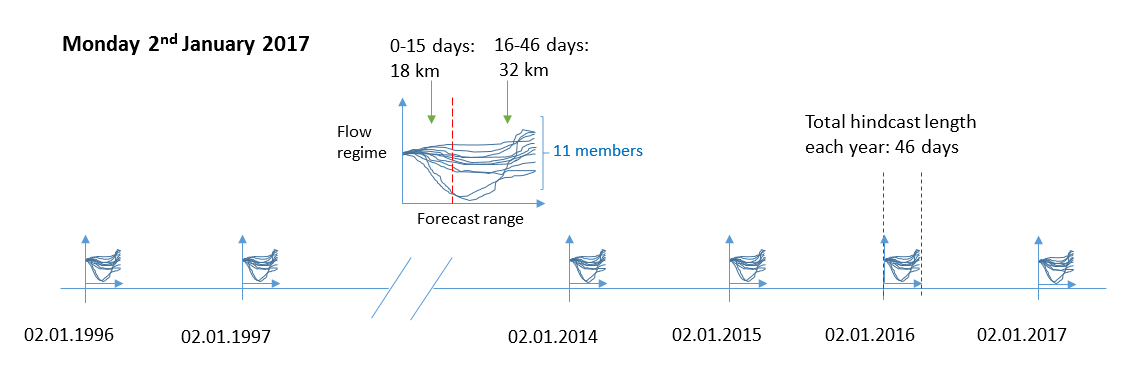
\includegraphics[width=34pc,angle=0]{ec_hindcast2.png}
	\caption{An example of the ECMWF hindcast schedule. For example, on Monday 2nd January 2017, 20 hindcast years (back to 1996) will be run. Each ensemble is made up of 11 members that reduce in resolution at day 15. (or day 10?) and run for a total of 46 days.}\label{fig:ecmwf_hindcast}
	\centering
\end{figure}

Over a year, with a model run on every Monday and Thursday for ... days, an entire 20 year period with xxx ensembles will have been created.

Hindcasts are a useful product to use......

A hindcast, or reforecast is a model forecast run initialised with conditions in the past. The hindcast run commences every Monday and Thursday, for that day for the past 20 years (to 1996) (figure \ref{fig:hindcast}).


Over a year, with a model run on every Monday and Thursday, an entire 20 year period with 10 ensembles members plus the control will have been created. Resolution of all of the members decreases at day 16. The initial 15 days of the hindcast that are analysed here have a resolution of 0.2$^0$. The ensemble members have five different ocean temperature analyses, with members 1 and 6, 2 and 7, 3 and 8, 4 and 9, 5 and 10 sharing the same initial state. These perturbed states are produced by adding randomly chosen wind perturbations to the ocean data assimilation, driven by five slightly different meteorological fields based on the control analysis.

For the ocean, we use 5 different ocean re-analyses (control + 4 perturbed) which are used to perturb the 11 members - which means that there are pairs of members which share the same SSTs as you said.

atmosphere: Singular vectors are applied in the Extratropics + Ensemble data assimilation (EDA) perturbations everywhere.

No, the atmospheric model is also perturbed using stochastic perturbations (SPPT scheme and also back-scatter scheme for the model version you are using), but only for the perturbed forecasts. The control forecast (type  cf or ensemble 0) is not perturbed. 

(Frederic email 9 Nov)
%What about the different atmosphere or model parts?
%The current version of the ECMWF model is given .. data based on xx of a day in the past and then runs forwards as a forecast. This provides a way to calibrate the output.
%Skill evaluation and calibration - the model drifts, so need to estimate from the model climate. Do not issue forecasts directly from the model, use anomalies.
%Reforecasts initialised from ERA-Interim, not OSTIA.

%% Analysis and model physics perturbed  https://www.ecmwf.int/en/forecasts/documentation-and-support#reforecasts
%ensemble members lower res???  na... all 18 km ??
%


\subsubsection {Operational forecast}  \label{ECMWF_forecast}
The high resolution (deterministic) operational forecast uses an atmosphere-only GCM. SSTs come from the Operational Sea Surface Temperature and Sea Ice Analysis (OSTIA) analysis at day 0, which persist throughout the forecast window (days 0-10). This is a high resolution analysis of the SST for the global ocean with daily, global coverage 1/20$^0$ ($\tilde{6}$ km) combined SST and sea ice concentration product, which is generated in near real time \citep{donlon2012operational}.

\begin{table}%[h]
	\caption{Operational forecast resolution}\label{t_ecmwf2}
	%	\begin{center}
	%	\begin{tabular}{cccccccc} use p to wrap text
	\begin{tabular}{ ccc }
		\hline\hline
		Date & Grid & Horizontal resolution \\
		\hline\hline
		21.11.00 & N256 & 0.5$^0$ \textasciitilde{40} km \\ %% $ $ is math mode - put this around the bits that are not text
		01.02.06 & N400 & 0.225$^0$ \textasciitilde{25} km \\ %% $ $ is math mode - put this around the bits that are not text
		26.01.10 & N640 & 0.125$^0$ \textasciitilde{16} km \\ %% $ $ is math mode - put this around the bits that are not text
		08.03.16 & O1280 & 0.1$^0$ \textasciitilde{9} km \\ %% $ $ is math mode - put this around the bits that are not text		
		\hline
	\end{tabular}
	%\end{center}
\end{table}

The grid used for the operational forecasts is updated every \textasciitilde{6} years and is currently being run at 0.1$^0$ resolution (table \ref{t_ecmwf2}).
%What is the spectral resolution??
%
%The sst and sea ice are updated during the model integration according to the tendency obtained from climatology of OSTIA (5km) \citep{ecmwf_user_guide}.
%
%The ensemble forecast (days 0-10) is at half the horizontal resolution and also has fewer levels in the vertical.  During these initial 10 days, the forecast uses an atmosphere-only GCM, with OSTIA SSTs. Five different ocean analyses are distributed amongst the control and ensemble members, produced by adding wind perturbations from different meteorological fields. \citep{ecmwf_user_guide}.  From days 10-46, the horizontal resolution of the ensemble is reduced to half (to 32 km) and the atmosphere is coupled to the NEMO ocean model \citep{madec2015nemo}. 
%The 50 ensemble members are formed by making small changes to the 4D-VAR analysis, creating perturbed initial states \citep{ecmwf_user_guide}.
%
%How are the ensembles generated - different ocean initial state and atmospheric initial state??
%
%ensemble forecast:
%The horizontal resolution of the ensemble is reduced at day 10, and the remainder of the forecast (out to 15 or 32 days) is run at half the resolution of the first 10 days.
%No ocean coupling for the first 10 days. From day 10 onwards, coupled to ocean model (5 ocean analyses for initial conditions).
%
%
%"The ocean-atmosphere coupling is achieved by a two-way interaction: the atmosphere affects the ocean through its wind, heat and net precipitation (precip-evap), whilst the ocean affects the atmosphere through its SST. for the ENS, this interaction is every hour" \citep{ecmwf_user_guide}.
%
%With respect to synoptic patterns, the control ensemble forecast  gives a similar performance to HRES, which is at twice the resolution \citep{ecmwf_user_guide}. However, HRES is better at forecasting small-scale extreme events, for example strong winds and heavy rain, when resolution is more important. 
%
%The high resolution model will be coupled to NEMO 0.25$^0$ at the end of 2017.
%Verification against ERA-Interim.
%Archived at the resolution run at.


The high resolution (deterministic) operational forecast uses an atmosphere-only GCM. SSTS come from the Operational Sea Surface Temperature and Sea Ice Analysis (OSTIA) analysis at day 0, which persist throughout the forecast window (days 0-10). This is a high resolution analysis of the SST for the global ocean with daily, global coverage 1/20° (~6 km) combined SST and sea ice concentration product, which is generated in near real time \citep{donlon2012operational}.
What is the spectral resolution??

The sst and sea ice are updated during the model integration according to the tendency obtained from climatology of OSTIA (5km) \citep{ecmwf_user_guide}.

The ensemble forecast (days 0-10) is at half the horizontal resolution ( x compared to x) and also has fewer levels in the vertical.  During these initial 10 days, the forecast uses an atmosphere-only GCM, with OSTIA SSTs. Five different ocean analyses are distributed amongst the control and ensemble members, produced by adding wind perturbations from different meteorological fields. \citep{ecmwf_user_guide}.  From days 10-46, the horizontal resolution of the ensemble is reduced to half (to 32 km) and the atmosphere is coupled to the NEMO ocean model \citep{madec2015nemo}. 
The 50 ensemble members are formed by making small changes to the 4D-VAR analysis, creating perturbed initial states \citep{ecmwf_user_guide}.

How are the ensembles generated - different ocean initial state and atmospheric initial state??

ensemble forecast:
The horizontal resolution of the ensemble is reduced at day 10, and the remainder of the forecast (out to 15 or 32 days) is run at half the resolution of the first 10 days.
No ocean coupling for the first 10 days. From day 10 onwards, coupled to ocean model (5 ocean analyses for initial conditions).


"The ocean-atmosphere coupling is achieved by a two-way interaction: the atmosphere affects the ocean through its wind, heat and net precipitation (precip-evap), whilst the ocean affects the atmosphere through its SST. for the ENS, this interaction is every hour" \citep{ecmwf_user_guide}.

With respect to synoptic patterns, the control ensemble forecast  gives a similar performance to HRES, which is at twice the resolution \citep{ecmwf_user_guide}. However, HRES is better at forecasting small-scale extreme events, for example strong winds and heavy rain, when resolution is more important. 

The high resolution model will be coupled to NEMO 0.25$^0$ at the end of 2017.
Verification against ERA-Interim.
Archived at the resolution run at.


\begin{table}%[h]
	\caption{Operational forecast resolution}\label{t_ecmwf2}
	%	\begin{center}
	%	\begin{tabular}{cccccccc} use p to wrap text
	\begin{tabular}{ ccc }
		\hline\hline
		Date & Grid & Horizontal resolution \\
		\hline\hline
		21.11.00 & N256 & 0.5$^0$ \textasciitilde{40} km \\ %% $ $ is math mode - put this around the bits that are not text
		01.02.06 & N400 & 0.225$^0$ \textasciitilde{25} km \\ %% $ $ is math mode - put this around the bits that are not text
		26.01.10 & N640 & 0.125$^0$ \textasciitilde{16} km \\ %% $ $ is math mode - put this around the bits that are not text
		08.03.16 & O1280 & 0.1$^0$ \textasciitilde{9} km \\ %% $ $ is math mode - put this around the bits that are not text		
		\hline
	\end{tabular}
	%\end{center}
\end{table}

The grid used for the operational forecasts is updated every \textasciitilde{6} years and is currently being run at 0.1$^0$ resolution (table \ref{t_ecmwf2}).
%What is the spectral resolution??
%
%The sst and sea ice are updated during the model integration according to the tendency obtained from climatology of OSTIA (5km) \citep{ecmwf_user_guide}.
%
%The ensemble forecast (days 0-10) is at half the horizontal resolution and also has fewer levels in the vertical.  During these initial 10 days, the forecast uses an atmosphere-only GCM, with OSTIA SSTs. Five different ocean analyses are distributed amongst the control and ensemble members, produced by adding wind perturbations from different meteorological fields. \citep{ecmwf_user_guide}.  From days 10-46, the horizontal resolution of the ensemble is reduced to half (to 32 km) and the atmosphere is coupled to the NEMO ocean model \citep{madec2015nemo}. 
%The 50 ensemble members are formed by making small changes to the 4D-VAR analysis, creating perturbed initial states \citep{ecmwf_user_guide}.
%
%How are the ensembles generated - different ocean initial state and atmospheric initial state??
%
%ensemble forecast:
%The horizontal resolution of the ensemble is reduced at day 10, and the remainder of the forecast (out to 15 or 32 days) is run at half the resolution of the first 10 days.
%No ocean coupling for the first 10 days. From day 10 onwards, coupled to ocean model (5 ocean analyses for initial conditions).
%
%
%"The ocean-atmosphere coupling is achieved by a two-way interaction: the atmosphere affects the ocean through its wind, heat and net precipitation (precip-evap), whilst the ocean affects the atmosphere through its SST. for the ENS, this interaction is every hour" \citep{ecmwf_user_guide}.
%
%With respect to synoptic patterns, the control ensemble forecast  gives a similar performance to HRES, which is at twice the resolution \citep{ecmwf_user_guide}. However, HRES is better at forecasting small-scale extreme events, for example strong winds and heavy rain, when resolution is more important. 
%
%The high resolution model will be coupled to NEMO 0.25$^0$ at the end of 2017.
%Verification against ERA-Interim.
%Archived at the resolution run at.

\subsubsection {ERA-Interim reanalysis}  \label{ECMWF_ERA}


\begin{table}[h]
	\caption{Variables}\label{t_variables}
	\begin{center}
		\begin{tabular}{ccc}
			
			\hline\hline
			$Variable$ & $Units$ & $Pressure Levels (hPa)$ \\
			\hline
			Zonal wind (u) & ms$^-1$ & 300, 400, 500, 700, 850, 925, 1000 \\ %% $ $ is math mode - put this around the bits that are not text
			Meridional wind (v) & ms$^-1$ & 300, 400, 500, 700, 850, 925, 1000  \\
			Vertical .. (w) & ms$^-1$ & 300, 400, 500, 700, 850, 925, 1000  \\
			Temperature (t) & K & 300, 400, 500, 700, 850, 925, 1000 \\
			Potential temperature (theta) & ms & 300, 400, 500, 700, 850, 925, 1000  \\
			q (q) & ms & 300, 400, 500, 700, 850, 925, 1000  \\
			Potential vorticity (PV) & ms & N/A  \\
			Geopotential height (Z) & ms & xx  \\
			
			\hline
		\end{tabular}
	\end{center}
\end{table}
% available at 50, 100, 200, 300, 400, 500, 700, 850, 925, 1000
Specific Humidity, Quasi-geostrophic Potential Vorticity, Water Vapor Mixing Ratio

At 6-hourly temporal resolution, time step 0 to 360, which is 10 days.

ERA-Interim is a global atmospheric reanalysis from 1979, continuously updated in real time. The spatial resolution of the data set is approximately 80 km (T255 spectral) on 60 vertical levels from the surface up to 0.1 hPa \citep{dee2011era}.

%http://www.ecmwf.int/en/research/modelling-and-prediction/atmospheric-dynamics
%"The wave model at ECMWF is called the “WAM”. It describes the rate of change of the 2- dimensional wave spectrum, in any water depth, caused by advection, wind input, dissipation due to white capping and bottom friction and non-linear wave interactions. It is set up so as to allow the two-way interaction of wind and waves with the atmospheric model. It is also incorporated in the medium-range, monthly and seasonal ensembles. 
%Radar altimeter wave-height data are assimilated from satellites. Buoy wave data are not assimilated; instead, they serve as an independent check on the quality of modelled wave parameters. The propagation of swell in the wave model is handled by a simple scheme that gives rise to a smoothing of the wave field. At present the effects of surface currents on the sea state are not taken into account. In particular areas, such as the Gulf Stream or Agulhas current, the current effect may give rise to localised changes of up to one metre in the wave height. The representation of the sea-ice fields is not as accurate as would be needed to handle waves near the ice edge. Due to the present model resolution, wave products near the coasts and, to a lesser extent, in small enclosed basins (e.g. the Baltic Sea) may be of lower quality than the open-ocean products. "
%Tides?

"The OGCM can reproduce the general features of the circulation and the thermal structure of the upper layers of the ocean and its seasonal, but has systematic errors, some of which are caused by the coarse vertical and horizontal resolution: the model thermocline is too diffuse; the Gulf Stream does not separate at the right location. (ref online guide).
The ocean analysis is performed every 10 days, down to a depth of 2000 m. The ocean-atmosphere coupling is achieved by a two-way interaction: the atmosphere affects the ocean through its wind, heat and net precipitation (precipitation-evaporation), whilst the ocean affects the atmosphere through its SST. For ENS, this interaction is every hour. what about regular forecast? not needed?? "


\begin{figure}
	
	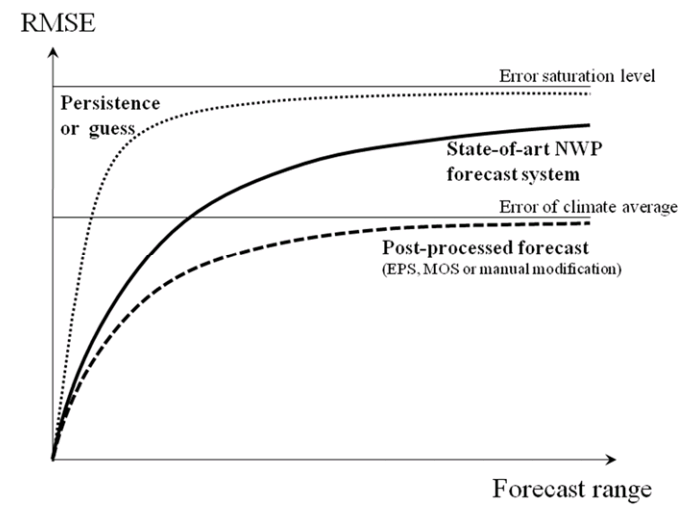
\includegraphics[width=22pc,angle=0]{forecast_error.png}
	\caption{Forecast error. From ECMWF web guide}\label{fig:forecast_error}
	\centering
\end{figure}


More details about spectral and truncation. Spectral and grids...
Parametrisation scheme...
global
hydrostatic - pressure coordinates?

%I will be looking at the medium-range(3-10 days). ECMWF’s forecasts cover time frames ranging from medium-range (3-10 days), to monthly and seasonal, and up to a year ahead.
%Nowcasting (0 - 6 hours)
%Short-range weather forecasts (1 - 3 days)
%Medium-range weather forecasts (3 - 10 days)

%"Between day 9 and day 10 there is a 24-hour overlap period, to reduce the “shock” of the change, in particular for the parameters that are most sensitive, for example convection and large-scale precipitation. Accumulations of precipitation (and other fluxes) for periods that span the resolution change (day 10) need to use low-resolution data from the overlap period and such data is thereforeavailable via dissemination."

%Not dealt with 'Forecasts from 15 to 32 days'

ERA-5 reanalysis download at 0.25 degree resolution
https://software.ecmwf.int/wiki/display/CKB/ERA5+data+documentation

% https://software.ecmwf.int/wiki/display/CKB/Does+downloading+data+at+higher+resolution+improve+the+output

For ERA-Interim the point interval on the native Gaussian grid is about 0.75 degrees (with the exception of Ocean-Wave data which are natively stored on the wave model’s reduced 1.0x1.0 degrees latitude/longitude grid). You can specify a custom grid on the data server web interface, or using the ECMWF WebAPI or using the MARS client (if you have access to it).  On the web interface the default grid for ERA-Interim is lat/long, with a default resolution of 0.75x0.75 degrees (about 80km), approximating the irregular grid spacing on the native Gaussian grid.

For ERA5 data the point interval on the native Gaussian grid is about 0.28 degrees. You can download ERA5 data using Python and specify a custom grid and resolution in your script. You should set the horizontal resolution to slightly lower than 0.28 degrees (about 30km), for example to 0.25 degrees, approximating the irregular grid spacing on the native Gaussian grid.



\subsection{Ensemble forecasting}

A hindcast, or reforecast is a model forecast run initialised with conditions in the past. The hindcast run commences every Monday and Thursday, for that day for the past 20 years (to 1996) (figure \ref{fig:hindcast}).

\begin{figure} [h]
	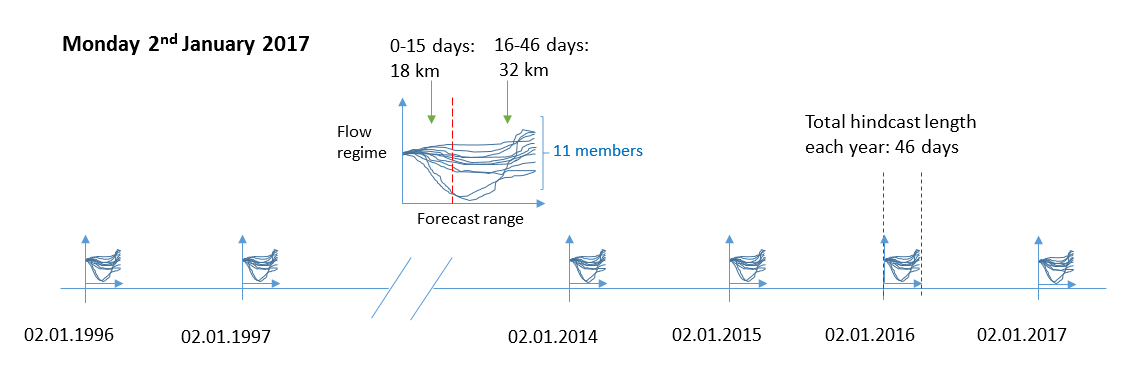
\includegraphics[width=34pc,angle=0]{ec_hindcast2.png}
	\caption{An example of the ECMWF hindcast schedule. For example, on Monday 2nd January 2017, 20 hindcast years (back to 1996) will be run. Each ensemble is made up of 11 members that reduce in resolution at day 15 and run for a total of 46 days.}\label{fig:ecmwf_hindcast}
	\centering
\end{figure} \label{fig:hindcast}	

Over a year, with a model run on every Monday and Thursday, an entire 20 year period with 10 ensembles members plus the control will have been created. Resolution of all of the members decreases at day 16. The initial 15 days of the hindcast that are analysed here have a resolution of 0.2$^0$. The ensemble members have five different ocean temperature analyses, with members 1 and 6, 2 and 7, 3 and 8, 4 and 9, 5 and 10 sharing the same initial state. These perturbed states are produced by adding randomly chosen wind perturbations to the ocean data assimilation, driven by five slightly different meteorological fields based on the control analysis.

For the ocean, we use 5 different ocean re-analyses (control + 4 perturbed) which are used to perturb the 11 members - which means that there are pairs of members which share the same SSTs as you said.

atmosphere: Singular vectors are applied in the Extratropics + Ensemble data assimilation (EDA) perturbations everywhere.

No, the atmospheric model is also perturbed using stochastic perturbations (SPPT scheme and also back-scatter scheme for the model version you are using), but only for the perturbed forecasts. The control forecast (type  cf or ensemble 0) is not perturbed. 

(Frederic email 9 Nov)
%What about the different atmosphere or model parts?
%The current version of the ECMWF model is given .. data based on xx of a day in the past and then runs forwards as a forecast. This provides a way to calibrate the output.
%Skill evaluation and calibration - the model drifts, so need to estimate from the model climate. Do not issue forecasts directly from the model, use anomalies.
%Reforecasts initialised from ERA-Interim, not OSTIA.

%% Analysis and model physics perturbed  https://www.ecmwf.int/en/forecasts/documentation-and-support#reforecasts
%ensemble members lower res???  na... all 18 km ??
%
%Hindcasts are a useful product to use......


Poor forecasts result from errors in initial conditions and model errors, with initial conditions dominating during the first five days or so. "Analysis errors amplify most easily in the sensitive parts of the
atmosphere, in particular where strong baroclinic systems develop. These errors then move
downstream and amplify and thereby affect the large-scale flow. To estimate the effect of
possible initial analysis errors and the consequent uncertainty of the forecasts, small changes
to the 4D-Var analysis are made, creating an ensemble of many (currently 50) different,
“perturbed”, initial states. Model deficiencies are represented by a stochastic process. In order
to save computational time, the ensemble members are run with a lower resolution version of
the IFS. 
If the ensembles agree, it is a predictable state. If diverge significantly from each other and the control, less certain forecast. Also calculate the ensemble mean (EM). ENS provides information from which the probability of alternative
developments is calculated, in particular those related to risk of extreme or high-impact
weather. The three methods for creating the ensemble...

%\begin{figure}
%	
%	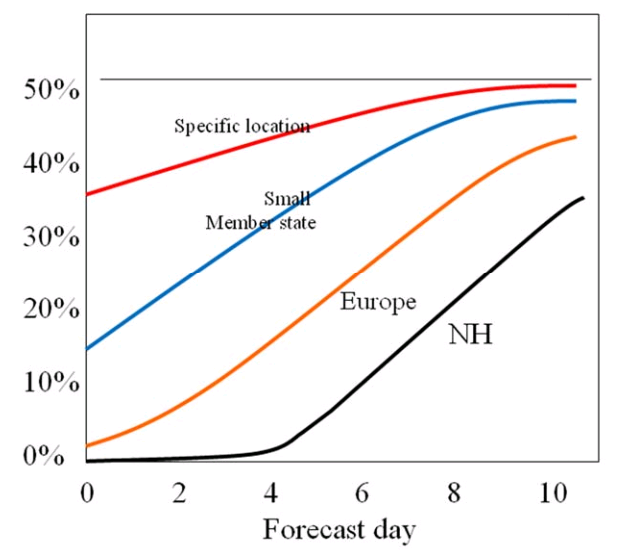
\includegraphics[width=22pc,angle=0]{H:/Documents/Thesis/phd-thesis-template-2.2.2_AC/phd-thesis-template-2.2.2/Figs/ens_pert.png}
%	\caption{Ensemble perturbation}\label{fig:ens_pert}
%	\centering
%\end{figure}

\begin{figure}
	
	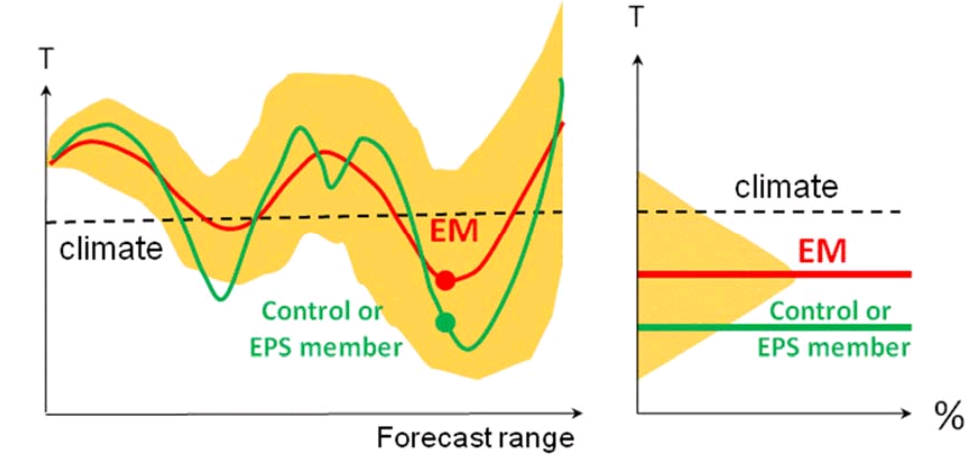
\includegraphics[width=22pc,angle=0]{ens_spread.png}
	\caption{Ensemble spread}\label{fig:ens_spread}
	\centering
\end{figure}

minobe2010atmospheric
kelly2010western
kwon2010role
Molteni, Corti, Palmer, Mike Wallace

%\subsection{The North Atlantic Oscillation}


\subsubsection {ERA5 reanalysis}  \label{ECMWF_ERA5}
% https://software.ecmwf.int/wiki/display/CKB/What+is+ERA5
ERA5 is the 5th major global reanalysis produced by ECMWF.
ERA5 uses the same 37 pressure levels as ERA-Interim.
All parameters available in ERA-Interim are also available in ERA5; and ERA5 has some additional parameters.
10 ensemble members, and also ensemble mean and spread for all parameters and levels are being produced. The temporal resolution is 3-hourly, rather than hourly for the deterministic ERA5 product, though.

%%%%%%%%%%%%%%%%%%%%%%%%%%%%%%%%%%%%%%%%%%%%%%%%%%%%%%%%%%%%%%%%%%%%%%
